\documentclass[twoside]{book}

% Packages required by doxygen
\usepackage{fixltx2e}
\usepackage{calc}
\usepackage{doxygen}
\usepackage[export]{adjustbox} % also loads graphicx
\usepackage{graphicx}
\usepackage[utf8]{inputenc}
\usepackage{makeidx}
\usepackage{multicol}
\usepackage{multirow}
\PassOptionsToPackage{warn}{textcomp}
\usepackage{textcomp}
\usepackage[nointegrals]{wasysym}
\usepackage[table]{xcolor}

% Font selection
\usepackage[T1]{fontenc}
\usepackage[scaled=.90]{helvet}
\usepackage{courier}
\usepackage{amssymb}
\usepackage{sectsty}
\renewcommand{\familydefault}{\sfdefault}
\allsectionsfont{%
  \fontseries{bc}\selectfont%
  \color{darkgray}%
}
\renewcommand{\DoxyLabelFont}{%
  \fontseries{bc}\selectfont%
  \color{darkgray}%
}
\newcommand{\+}{\discretionary{\mbox{\scriptsize$\hookleftarrow$}}{}{}}

% Page & text layout
\usepackage{geometry}
\geometry{%
  a4paper,%
  top=2.5cm,%
  bottom=2.5cm,%
  left=2.5cm,%
  right=2.5cm%
}
\tolerance=750
\hfuzz=15pt
\hbadness=750
\setlength{\emergencystretch}{15pt}
\setlength{\parindent}{0cm}
\setlength{\parskip}{3ex plus 2ex minus 2ex}
\makeatletter
\renewcommand{\paragraph}{%
  \@startsection{paragraph}{4}{0ex}{-1.0ex}{1.0ex}{%
    \normalfont\normalsize\bfseries\SS@parafont%
  }%
}
\renewcommand{\subparagraph}{%
  \@startsection{subparagraph}{5}{0ex}{-1.0ex}{1.0ex}{%
    \normalfont\normalsize\bfseries\SS@subparafont%
  }%
}
\makeatother

% Headers & footers
\usepackage{fancyhdr}
\pagestyle{fancyplain}
\fancyhead[LE]{\fancyplain{}{\bfseries\thepage}}
\fancyhead[CE]{\fancyplain{}{}}
\fancyhead[RE]{\fancyplain{}{\bfseries\leftmark}}
\fancyhead[LO]{\fancyplain{}{\bfseries\rightmark}}
\fancyhead[CO]{\fancyplain{}{}}
\fancyhead[RO]{\fancyplain{}{\bfseries\thepage}}
\fancyfoot[LE]{\fancyplain{}{}}
\fancyfoot[CE]{\fancyplain{}{}}
\fancyfoot[RE]{\fancyplain{}{\bfseries\scriptsize Generated by Doxygen }}
\fancyfoot[LO]{\fancyplain{}{\bfseries\scriptsize Generated by Doxygen }}
\fancyfoot[CO]{\fancyplain{}{}}
\fancyfoot[RO]{\fancyplain{}{}}
\renewcommand{\footrulewidth}{0.4pt}
\renewcommand{\chaptermark}[1]{%
  \markboth{#1}{}%
}
\renewcommand{\sectionmark}[1]{%
  \markright{\thesection\ #1}%
}

% Indices & bibliography
\usepackage{natbib}
\usepackage[titles]{tocloft}
\setcounter{tocdepth}{3}
\setcounter{secnumdepth}{5}
\makeindex

% Hyperlinks (required, but should be loaded last)
\usepackage{ifpdf}
\ifpdf
  \usepackage[pdftex,pagebackref=true]{hyperref}
\else
  \usepackage[ps2pdf,pagebackref=true]{hyperref}
\fi
\hypersetup{%
  colorlinks=true,%
  linkcolor=blue,%
  citecolor=blue,%
  unicode%
}

% Custom commands
\newcommand{\clearemptydoublepage}{%
  \newpage{\pagestyle{empty}\cleardoublepage}%
}

\usepackage{caption}
\captionsetup{labelsep=space,justification=centering,font={bf},singlelinecheck=off,skip=4pt,position=top}

%===== C O N T E N T S =====

\begin{document}

% Titlepage & ToC
\hypersetup{pageanchor=false,
             bookmarksnumbered=true,
             pdfencoding=unicode
            }
\pagenumbering{alph}
\begin{titlepage}
\vspace*{7cm}
\begin{center}%
{\Large ssme }\\
\vspace*{1cm}
{\large Generated by Doxygen 1.8.13}\\
\end{center}
\end{titlepage}
\clearemptydoublepage
\pagenumbering{roman}
\tableofcontents
\clearemptydoublepage
\pagenumbering{arabic}
\hypersetup{pageanchor=true}

%--- Begin generated contents ---
\chapter{S\+S\+ME\+: a c++ static library for the estimation of state space models}
\label{index}\hypertarget{index}{}\href{https://zenodo.org/badge/latestdoi/154373836}{\tt }

The current availability includes\+:


\begin{DoxyEnumerate}
\item particle marginal Metropolis-\/\+Hastings with generic parameter proposal distributions.
\item particle marginal Metropolis-\/\+Hastings with multivariate normal random-\/walk proposals.
\end{DoxyEnumerate}

Also included is the {\ttfamily \hyperlink{classparamPack}{param\+Pack}} container class that holds onto parameters. Because it is quite common to transform the parameters, this class has the ability to return transformed and untransformed parameters vectors, as well as automatically compute and return (log-\/ )jacobians (which comes in handy when working with evaluating the parameter proposal distribution).

\subsection*{example\+:}

For an example, navigate to the {\ttfamily ssme/example} directory, type {\ttfamily make}, and then something like


\begin{DoxyCode}
./main spy\_returns.csv univ\_svol\_pmmh\_samples univ\_svol\_pmmh\_messages 1000
\end{DoxyCode}
 
\chapter{Hierarchical Index}
\section{Class Hierarchy}
This inheritance list is sorted roughly, but not completely, alphabetically\+:\begin{DoxyCompactList}
\item \contentsline{section}{ada\+\_\+pmmh$<$ numparams, dimobs, numparts $>$}{\pageref{classada__pmmh}}{}
\item \contentsline{section}{ada\+\_\+pmmh\+\_\+mvn$<$ numparams, dimobs, numparts $>$}{\pageref{classada__pmmh__mvn}}{}
\begin{DoxyCompactList}
\item \contentsline{section}{univ\+\_\+svol\+\_\+estimator$<$ numparams, dimnss, dimss, dimobs, numparts $>$}{\pageref{classuniv__svol__estimator}}{}
\end{DoxyCompactList}
\item B\+S\+Filter\begin{DoxyCompactList}
\item \contentsline{section}{svol\+\_\+bs$<$ nparts, dimx, dimy, resampT $>$}{\pageref{classsvol__bs}}{}
\end{DoxyCompactList}
\item \contentsline{section}{param\+Inv\+Transform}{\pageref{classparamInvTransform}}{}
\item \contentsline{section}{param\+Pack}{\pageref{classparamPack}}{}
\item \contentsline{section}{param\+Transform}{\pageref{classparamTransform}}{}
\begin{DoxyCompactList}
\item \contentsline{section}{logit\+Trans}{\pageref{classlogitTrans}}{}
\item \contentsline{section}{log\+Trans}{\pageref{classlogTrans}}{}
\item \contentsline{section}{null\+Trans}{\pageref{classnullTrans}}{}
\item \contentsline{section}{twice\+Fisher\+Trans}{\pageref{classtwiceFisherTrans}}{}
\end{DoxyCompactList}
\item rbpf\+\_\+hmm\+\_\+bs\begin{DoxyCompactList}
\item \contentsline{section}{msl1\+\_\+rbbpf$<$ nparts, dimnss, dimss, dimy, resampT $>$}{\pageref{classmsl1__rbbpf}}{}
\end{DoxyCompactList}
\end{DoxyCompactList}

\chapter{Class Index}
\doxysection{Class List}
Here are the classes, structs, unions and interfaces with brief descriptions\+:\begin{DoxyCompactList}
\item\contentsline{section}{\mbox{\hyperlink{classada__pmmh__mvn}{ada\+\_\+pmmh\+\_\+mvn$<$ numparams, dimobs, numparts, float\+\_\+t $>$}} }{\pageref{classada__pmmh__mvn}}{}
\item\contentsline{section}{\mbox{\hyperlink{classutils_1_1csv__param__sampler}{utils\+::csv\+\_\+param\+\_\+sampler$<$ dimparam, float\+\_\+t $>$}} }{\pageref{classutils_1_1csv__param__sampler}}{}
\item\contentsline{section}{\mbox{\hyperlink{classjoin__threads}{join\+\_\+threads}} \\*R\+A\+II thread killer }{\pageref{classjoin__threads}}{}
\item\contentsline{section}{\mbox{\hyperlink{classparam_1_1log__trans}{param\+::log\+\_\+trans$<$ float\+\_\+t $>$}} \\*Trans\+\_\+p = log(orig\+\_\+p) }{\pageref{classparam_1_1log__trans}}{}
\item\contentsline{section}{\mbox{\hyperlink{classparam_1_1logit__trans}{param\+::logit\+\_\+trans$<$ float\+\_\+t $>$}} \\*Trans\+\_\+p = logit(orig\+\_\+p) }{\pageref{classparam_1_1logit__trans}}{}
\item\contentsline{section}{\mbox{\hyperlink{classLWFilter}{L\+W\+Filter$<$ nparts, dimx, dimy, dimparam, float\+\_\+t, debug $>$}} \\*A base class for the Liu-\/\+West Filter }{\pageref{classLWFilter}}{}
\item\contentsline{section}{\mbox{\hyperlink{classLWFilter2}{L\+W\+Filter2$<$ nparts, dimx, dimy, dimparam, float\+\_\+t, debug $>$}} \\*A base class for a modified version of the Liu-\/\+West Filter }{\pageref{classLWFilter2}}{}
\item\contentsline{section}{\mbox{\hyperlink{classLWFilter2FutureSimulator}{L\+W\+Filter2\+Future\+Simulator$<$ nparts, dimx, dimy, dimparam, float\+\_\+t, debug $>$}} \\*An add-\/on for the Liu-\/\+West (version 2) Filter that simulates future observations }{\pageref{classLWFilter2FutureSimulator}}{}
\item\contentsline{section}{\mbox{\hyperlink{classLWFilter2WithCovs}{L\+W\+Filter2\+With\+Covs$<$ nparts, dimx, dimy, dimcov, dimparam, float\+\_\+t, debug $>$}} \\*A base class for a modified version of the Liu-\/\+West Filter. Unlike the above class, it allows the state transition to depend on covariates }{\pageref{classLWFilter2WithCovs}}{}
\item\contentsline{section}{\mbox{\hyperlink{classLWFilter2WithCovsFutureSimulator}{L\+W\+Filter2\+With\+Covs\+Future\+Simulator$<$ nparts, dimx, dimy, dimcov, dimparam, float\+\_\+t, debug $>$}} }{\pageref{classLWFilter2WithCovsFutureSimulator}}{}
\item\contentsline{section}{\mbox{\hyperlink{classLWFilterFutureSimulator}{L\+W\+Filter\+Future\+Simulator$<$ nparts, dimx, dimy, dimparam, float\+\_\+t, debug $>$}} \\*An add-\/on for the Liu-\/\+West Filter that simulates future observations }{\pageref{classLWFilterFutureSimulator}}{}
\item\contentsline{section}{\mbox{\hyperlink{classLWFilterWithCovs}{L\+W\+Filter\+With\+Covs$<$ nparts, dimx, dimy, dimcov, dimparam, float\+\_\+t, debug $>$}} \\*A base class for the Liu-\/\+West Filter. Unlike the above Liu-\/\+Wester filter base class, this allows the state transition to depend on covariates }{\pageref{classLWFilterWithCovs}}{}
\item\contentsline{section}{\mbox{\hyperlink{classLWFilterWithCovsFutureSimulator}{L\+W\+Filter\+With\+Covs\+Future\+Simulator$<$ nparts, dimx, dimy, dimcov, dimparam, float\+\_\+t, debug $>$}} \\*An add-\/on for the Liu-\/\+West Filter that simulates future observations }{\pageref{classLWFilterWithCovsFutureSimulator}}{}
\item\contentsline{section}{\mbox{\hyperlink{classmn__resamp__states__and__params}{mn\+\_\+resamp\+\_\+states\+\_\+and\+\_\+params$<$ nparts, dimx, dimparam, float\+\_\+t $>$}} }{\pageref{classmn__resamp__states__and__params}}{}
\item\contentsline{section}{\mbox{\hyperlink{classparam_1_1null__trans}{param\+::null\+\_\+trans$<$ float\+\_\+t $>$}} \\*Trans\+\_\+p = orig\+\_\+p }{\pageref{classparam_1_1null__trans}}{}
\item\contentsline{section}{\mbox{\hyperlink{classparam_1_1pack}{param\+::pack$<$ float\+\_\+t, numelem $>$}} \\*Stores transformed parameters, as well as the functions that can change them to the untransformed parameters and back }{\pageref{classparam_1_1pack}}{}
\item\contentsline{section}{\mbox{\hyperlink{classsplit__data__thread__pool}{split\+\_\+data\+\_\+thread\+\_\+pool$<$ dyn\+\_\+in\+\_\+t, static\+\_\+in\+\_\+elem\+\_\+t, out\+\_\+t, num\+\_\+static\+\_\+elems, debug $>$}} \\*Split data thread pool Unlike the above thread pool, this pre-\/allocates work across the nodes. \char`\"{}work\char`\"{} is initiated when there is a new object of type dyn\+\_\+in\+\_\+t, which is shared across all threads. Work is performed for every element of the array of static\+\_\+in\+\_\+elem\+\_\+t. The same function is applied to every pair }{\pageref{classsplit__data__thread__pool}}{}
\item\contentsline{section}{\mbox{\hyperlink{classsvol__bs}{svol\+\_\+bs$<$ nparts, dimx, dimy, resamp\+T, float\+\_\+t $>$}} }{\pageref{classsvol__bs}}{}
\item\contentsline{section}{\mbox{\hyperlink{classSwarm}{Swarm$<$ Mod\+Type, n\+\_\+filt\+\_\+funcs, nstateparts, nparamparts, dimy, dimx, dimparam $>$}} \\*Object that implements a \char`\"{}particle swarm filter\char`\"{} (see \href{https://arxiv.org/abs/2006.15396}{\texttt{ https\+://arxiv.\+org/abs/2006.\+15396}}) This class will draw parameters from samp\+\_\+untrans\+\_\+param (a pure virtual function). This function will usually draw from some distribution that closely approximates an old posterior, and it can even draw from posterior samples in another file }{\pageref{classSwarm}}{}
\item\contentsline{section}{\mbox{\hyperlink{classSwarmWithCovs}{Swarm\+With\+Covs$<$ Mod\+Type, n\+\_\+filt\+\_\+funcs, nstateparts, nparamparts, dimy, dimx, dimcov, dimparam, debug $>$}} }{\pageref{classSwarmWithCovs}}{}
\item\contentsline{section}{\mbox{\hyperlink{classthread__pool}{thread\+\_\+pool$<$ dyn\+\_\+data\+\_\+t, static\+\_\+data\+\_\+t, func\+\_\+output\+\_\+t, debug $>$}} \\*Here we have many concurrent parameter readers, but only a single parameter writer. This thread pool owns one function that returns one (random) floating point number. The pool sits ready to perform calculations on any new parameter value. Once a new parameter value is received, this pool calls its function a fixed number of times, and all of the function output is averaged in a thread-\/safe way. Actually, these function evals are expected to be in the log space, and the log-\/mean-\/exp is calculated using the log-\/sum-\/exp trick. For our particular applications, this function will also depend on observed data that doesn\textquotesingle{}t change once the thread pool has been initialized }{\pageref{classthread__pool}}{}
\item\contentsline{section}{\mbox{\hyperlink{classparam_1_1transform}{param\+::transform$<$ float\+\_\+t $>$}} \\*Pure virtual base class. cts params only }{\pageref{classparam_1_1transform}}{}
\item\contentsline{section}{\mbox{\hyperlink{classparam_1_1twice__fisher__trans}{param\+::twice\+\_\+fisher\+\_\+trans$<$ float\+\_\+t $>$}} \\*Trans\+\_\+p = log(1+orig\+\_\+p) -\/ log(1-\/orig\+\_\+p) = logit((orig\+\_\+p+1)/2) }{\pageref{classparam_1_1twice__fisher__trans}}{}
\item\contentsline{section}{\mbox{\hyperlink{classuniv__svol__estimator}{univ\+\_\+svol\+\_\+estimator$<$ numparams, dimstate, dimobs, numparts, float\+\_\+t $>$}} }{\pageref{classuniv__svol__estimator}}{}
\end{DoxyCompactList}

\chapter{File Index}
\section{File List}
Here is a list of all documented files with brief descriptions\+:\begin{DoxyCompactList}
\item\contentsline{section}{example/{\bfseries estimate\+\_\+univ\+\_\+svol.\+h} }{\pageref{estimate__univ__svol_8h}}{}
\item\contentsline{section}{example/{\bfseries univ\+\_\+svol\+\_\+bootstrap\+\_\+filter.\+h} }{\pageref{univ__svol__bootstrap__filter_8h}}{}
\item\contentsline{section}{include/\hyperlink{ada__pmmh_8h}{ada\+\_\+pmmh.\+h} \\*Performs an adaptive version of the particle marginal Metropilis-\/\+Hastings algorithm. The user is asked to design his/her own proposal density and prior distribution. The sampling is handled on an \char`\"{}as-\/is\char`\"{} basis, which means that it is entirely the user\textquotesingle{}s own responsibility to decide on what parameterization to use, to handle Jacobians if they are necessary, etc. These parameters will be written in an \char`\"{}as-\/is\char`\"{} fashion, as well. These calculations can be facilitates using the {\ttfamily \hyperlink{classparamPack}{param\+Pack}} class, however using this class is not absolutely necessary. Also, for convenience, a moving average covariance matrix estimate is performed; however, this should be ignored if the user is not interested in adaptive M\+C\+MC or isn\textquotesingle{}t using a transformed parameter space }{\pageref{ada__pmmh_8h}}{}
\item\contentsline{section}{include/\hyperlink{ada__pmmh__mvn_8h}{ada\+\_\+pmmh\+\_\+mvn.\+h} \\*Performs adaptive particle marginal metropolis-\/hastings sampling, using a multivariate normal distribution as the proposal. This samples on the transformed space, but it writes out the untransformed/constrained samples to the output. The priors requested by the user are for the (hopefully more convenient) un-\/transformed or constrained space. This means that the user never has to worry about handling any kind of Jacobian--just specify a prior on the familiar space, and a function that approximates log-\/likelihoods }{\pageref{ada__pmmh__mvn_8h}}{}
\item\contentsline{section}{include/\hyperlink{ada__rwmh_8h}{ada\+\_\+rwmh.\+h} \\*Performs adaptive random walk metropolis-\/hastings sampling (uses a multivariate normal distribution as the proposal). This samples on the transformed space, but it writes the untransformed/constrained samples to the output. The priors requested by the user are for the (more convenient) un-\/transformed aka constrained space. This means that the user never has to worry about handling any kind of Jacobian }{\pageref{ada__rwmh_8h}}{}
\item\contentsline{section}{include/{\bfseries get\+\_\+mcmc\+\_\+estimate.\+h} }{\pageref{get__mcmc__estimate_8h}}{}
\item\contentsline{section}{include/\hyperlink{param__pack_8h}{param\+\_\+pack.\+h} \\*Stores transformed parameters, as well as the functions that can change them to the untransformed parameters and back }{\pageref{param__pack_8h}}{}
\item\contentsline{section}{include/\hyperlink{param__transforms_8h}{param\+\_\+transforms.\+h} \\*Pure virtual base class. cts params only }{\pageref{param__transforms_8h}}{}
\end{DoxyCompactList}

\chapter{Class Documentation}
\hypertarget{classada__pmmh}{}\section{ada\+\_\+pmmh$<$ numparams, dimobs, numparts $>$ Class Template Reference}
\label{classada__pmmh}\index{ada\+\_\+pmmh$<$ numparams, dimobs, numparts $>$@{ada\+\_\+pmmh$<$ numparams, dimobs, numparts $>$}}


{\ttfamily \#include $<$ada\+\_\+pmmh.\+h$>$}

\subsection*{Public Types}
\begin{DoxyCompactItemize}
\item 
\mbox{\Hypertarget{classada__pmmh_ad6cc974f0e1946b055e476893045c5e0}\label{classada__pmmh_ad6cc974f0e1946b055e476893045c5e0}} 
using {\bfseries osv} = Eigen\+::\+Matrix$<$ double, dimobs, 1 $>$
\item 
\mbox{\Hypertarget{classada__pmmh_a24849179e51b6cb08b39124b516d7268}\label{classada__pmmh_a24849179e51b6cb08b39124b516d7268}} 
using {\bfseries psv} = Eigen\+::\+Matrix$<$ double, numparams, 1 $>$
\item 
\mbox{\Hypertarget{classada__pmmh_acaa46542b8ebe093c93be5e086940b40}\label{classada__pmmh_acaa46542b8ebe093c93be5e086940b40}} 
using {\bfseries psm} = Eigen\+::\+Matrix$<$ double, numparams, numparams $>$
\end{DoxyCompactItemize}
\subsection*{Public Member Functions}
\begin{DoxyCompactItemize}
\item 
\hyperlink{classada__pmmh_a9e8c52947fd34c7d75f3397d64f586e4}{ada\+\_\+pmmh} (const psv \&start\+\_\+trans\+\_\+theta, const unsigned int \&num\+\_\+mcmc\+\_\+iters, const std\+::string \&data\+\_\+file, const std\+::string \&samples\+\_\+file, const std\+::string \&messages\+\_\+file, const bool \&mc, const unsigned int \&t0, const unsigned int \&t1, const psm \&C0)
\begin{DoxyCompactList}\small\item\em The constructor. \end{DoxyCompactList}\item 
psm \hyperlink{classada__pmmh_ae8cbd73ca691b9ad464c00ff666a8b48}{get\+\_\+ct} () const
\begin{DoxyCompactList}\small\item\em Get the current proposal distribution\textquotesingle{}s covariance matrix. \end{DoxyCompactList}\item 
\mbox{\Hypertarget{classada__pmmh_a06aeab11ff56e6d1d3c886e7ac2980f7}\label{classada__pmmh_a06aeab11ff56e6d1d3c886e7ac2980f7}} 
void \hyperlink{classada__pmmh_a06aeab11ff56e6d1d3c886e7ac2980f7}{commence\+Sampling} ()
\begin{DoxyCompactList}\small\item\em starts the sampling \end{DoxyCompactList}\item 
virtual double \hyperlink{classada__pmmh_a249575415a567c4f62e62e9864abd867}{log\+Prior\+Evaluate} (const psv \&trans\+Theta)=0
\begin{DoxyCompactList}\small\item\em Evaluates the log of the model\textquotesingle{}s prior distribution. \end{DoxyCompactList}\item 
virtual double \hyperlink{classada__pmmh_a64274a7a1a54b99fb10e53f3b09925eb}{log\+Q\+Evaluate} (const psv \&old\+Trans\+Params, const psv \&new\+Trans\+Params)=0
\begin{DoxyCompactList}\small\item\em Evaluates the logarithm of the proposal density. \end{DoxyCompactList}\item 
virtual double \hyperlink{classada__pmmh_ae07210fc64b1966cef4d5a594be687f1}{log\+Like\+Evaluate} (const psv \&trans\+Theta, const std\+::vector$<$ osv $>$ \&data, std\+::atomic\+\_\+bool \&cancelled)=0
\begin{DoxyCompactList}\small\item\em Approximates the log likelihood with a particle filter. \end{DoxyCompactList}\end{DoxyCompactItemize}
\subsection*{Private Member Functions}
\begin{DoxyCompactItemize}
\item 
\mbox{\Hypertarget{classada__pmmh_adddc585ea12dec19e3ac3c03d5c56d2e}\label{classada__pmmh_adddc585ea12dec19e3ac3c03d5c56d2e}} 
void {\bfseries update\+\_\+moments\+\_\+and\+\_\+\+Ct} (const psv \&new\+Trans\+Theta)
\item 
\mbox{\Hypertarget{classada__pmmh_aad55e7f0dc8dbfa1ffff00d9d855a081}\label{classada__pmmh_aad55e7f0dc8dbfa1ffff00d9d855a081}} 
psv {\bfseries q\+Sample} (const psv \&old\+Trans\+Theta)
\end{DoxyCompactItemize}
\subsection*{Private Attributes}
\begin{DoxyCompactItemize}
\item 
\mbox{\Hypertarget{classada__pmmh_a4eae8f5350ee02b3041a56b8477b7cc9}\label{classada__pmmh_a4eae8f5350ee02b3041a56b8477b7cc9}} 
std\+::vector$<$ osv $>$ {\bfseries m\+\_\+data}
\item 
\mbox{\Hypertarget{classada__pmmh_ab95501d2b47c94e405959545094b33c4}\label{classada__pmmh_ab95501d2b47c94e405959545094b33c4}} 
psv {\bfseries m\+\_\+current\+\_\+trans\+\_\+theta}
\item 
\mbox{\Hypertarget{classada__pmmh_a4397034d42abf48d85c37573ad4b137a}\label{classada__pmmh_a4397034d42abf48d85c37573ad4b137a}} 
psm {\bfseries m\+\_\+sigma\+\_\+hat}
\item 
\mbox{\Hypertarget{classada__pmmh_af92a45bb0f1c09695f9bdfe70da91268}\label{classada__pmmh_af92a45bb0f1c09695f9bdfe70da91268}} 
psv {\bfseries m\+\_\+mean\+\_\+trans\+\_\+theta}
\item 
\mbox{\Hypertarget{classada__pmmh_a7257a454e068ef74880f166b0d1e73d5}\label{classada__pmmh_a7257a454e068ef74880f166b0d1e73d5}} 
double {\bfseries m\+\_\+ma\+\_\+accept\+\_\+rate}
\item 
\mbox{\Hypertarget{classada__pmmh_a70197ecca3a74968e814a45261052b72}\label{classada__pmmh_a70197ecca3a74968e814a45261052b72}} 
unsigned int {\bfseries m\+\_\+t0}
\item 
\mbox{\Hypertarget{classada__pmmh_a4e2f07d2dfc87db3db46dda6f3e0b3e1}\label{classada__pmmh_a4e2f07d2dfc87db3db46dda6f3e0b3e1}} 
unsigned int {\bfseries m\+\_\+t1}
\item 
\mbox{\Hypertarget{classada__pmmh_a75a274ef04d45f7f6bb3c444bf063c2c}\label{classada__pmmh_a75a274ef04d45f7f6bb3c444bf063c2c}} 
psm {\bfseries m\+\_\+\+Ct}
\item 
\mbox{\Hypertarget{classada__pmmh_ad1f3dabd5006b89a899c8ae2daad169f}\label{classada__pmmh_ad1f3dabd5006b89a899c8ae2daad169f}} 
rvsamp\+::\+M\+V\+N\+Sampler$<$ numparams $>$ {\bfseries m\+\_\+mvn\+\_\+gen}
\item 
\mbox{\Hypertarget{classada__pmmh_a16e7aea5b2b3d77514e62c878cd3a906}\label{classada__pmmh_a16e7aea5b2b3d77514e62c878cd3a906}} 
std\+::ofstream {\bfseries m\+\_\+samples\+\_\+file\+\_\+stream}
\item 
\mbox{\Hypertarget{classada__pmmh_a925dfc2e2fcd61bd37db705f5c894a1b}\label{classada__pmmh_a925dfc2e2fcd61bd37db705f5c894a1b}} 
std\+::ofstream {\bfseries m\+\_\+message\+\_\+stream}
\item 
\mbox{\Hypertarget{classada__pmmh_a8207d3f7daf94a467ae33c9261256379}\label{classada__pmmh_a8207d3f7daf94a467ae33c9261256379}} 
unsigned int {\bfseries m\+\_\+num\+\_\+mcmc\+\_\+iters}
\item 
\mbox{\Hypertarget{classada__pmmh_a17938a6b9f5e737de9d93b9c82583597}\label{classada__pmmh_a17938a6b9f5e737de9d93b9c82583597}} 
unsigned int {\bfseries m\+\_\+num\+\_\+extra\+\_\+threads}
\item 
\mbox{\Hypertarget{classada__pmmh_a4e7a7f0ef7a203002c8585c7135e753d}\label{classada__pmmh_a4e7a7f0ef7a203002c8585c7135e753d}} 
bool {\bfseries m\+\_\+multicore}
\item 
\mbox{\Hypertarget{classada__pmmh_a271d36e458c9067e518d31f27f6fe493}\label{classada__pmmh_a271d36e458c9067e518d31f27f6fe493}} 
unsigned int {\bfseries m\+\_\+iter}
\item 
\mbox{\Hypertarget{classada__pmmh_ac19f1f8da164c84937d890026729035e}\label{classada__pmmh_ac19f1f8da164c84937d890026729035e}} 
double {\bfseries m\+\_\+sd}
\item 
\mbox{\Hypertarget{classada__pmmh_ac50a7d1c54985b3468b5384a33e321ef}\label{classada__pmmh_ac50a7d1c54985b3468b5384a33e321ef}} 
double {\bfseries m\+\_\+eps}
\end{DoxyCompactItemize}


\subsection{Detailed Description}
\subsubsection*{template$<$size\+\_\+t numparams, size\+\_\+t dimobs, size\+\_\+t numparts$>$\newline
class ada\+\_\+pmmh$<$ numparams, dimobs, numparts $>$}

\begin{DoxyAuthor}{Author}
t 
\end{DoxyAuthor}


\subsection{Constructor \& Destructor Documentation}
\mbox{\Hypertarget{classada__pmmh_a9e8c52947fd34c7d75f3397d64f586e4}\label{classada__pmmh_a9e8c52947fd34c7d75f3397d64f586e4}} 
\index{ada\+\_\+pmmh@{ada\+\_\+pmmh}!ada\+\_\+pmmh@{ada\+\_\+pmmh}}
\index{ada\+\_\+pmmh@{ada\+\_\+pmmh}!ada\+\_\+pmmh@{ada\+\_\+pmmh}}
\subsubsection{\texorpdfstring{ada\+\_\+pmmh()}{ada\_pmmh()}}
{\footnotesize\ttfamily template$<$size\+\_\+t numparams, size\+\_\+t dimobs, size\+\_\+t numparts$>$ \\
\hyperlink{classada__pmmh}{ada\+\_\+pmmh}$<$ numparams, dimobs, numparts $>$\+::\hyperlink{classada__pmmh}{ada\+\_\+pmmh} (\begin{DoxyParamCaption}\item[{const psv \&}]{start\+\_\+trans\+\_\+theta,  }\item[{const unsigned int \&}]{num\+\_\+mcmc\+\_\+iters,  }\item[{const std\+::string \&}]{data\+\_\+file,  }\item[{const std\+::string \&}]{samples\+\_\+file,  }\item[{const std\+::string \&}]{messages\+\_\+file,  }\item[{const bool \&}]{mc,  }\item[{const unsigned int \&}]{t0,  }\item[{const unsigned int \&}]{t1,  }\item[{const psm \&}]{C0 }\end{DoxyParamCaption})}



The constructor. 


\begin{DoxyParams}{Parameters}
{\em start\+\_\+trans\+\_\+theta} & the initial (possibly transformed) parameters you want to start sampling from. \\
\hline
{\em num\+\_\+mcmc\+\_\+iters} & the number of M\+C\+MC iterations you want to do. \\
\hline
{\em data\+\_\+file} & the location of the observed time series data. \\
\hline
{\em samples\+\_\+file} & the location where you want to store the samples. \\
\hline
{\em messages\+\_\+file} & the location where you want to store the messages. \\
\hline
{\em mc} & stands for multicore. true or false if you want to use extra cores. \\
\hline
{\em t0} & iteration at which you start adapting the posterior covariance matrix. \\
\hline
{\em t1} & time you stop adapting the posterior covariance matrix. \\
\hline
{\em C0} & initial covariance matrix to be used in the moving ave. calculation. \\
\hline
\end{DoxyParams}


\subsection{Member Function Documentation}
\mbox{\Hypertarget{classada__pmmh_ae8cbd73ca691b9ad464c00ff666a8b48}\label{classada__pmmh_ae8cbd73ca691b9ad464c00ff666a8b48}} 
\index{ada\+\_\+pmmh@{ada\+\_\+pmmh}!get\+\_\+ct@{get\+\_\+ct}}
\index{get\+\_\+ct@{get\+\_\+ct}!ada\+\_\+pmmh@{ada\+\_\+pmmh}}
\subsubsection{\texorpdfstring{get\+\_\+ct()}{get\_ct()}}
{\footnotesize\ttfamily template$<$size\+\_\+t numparams, size\+\_\+t dimobs, size\+\_\+t numparts$>$ \\
auto \hyperlink{classada__pmmh}{ada\+\_\+pmmh}$<$ numparams, dimobs, numparts $>$\+::get\+\_\+ct (\begin{DoxyParamCaption}{ }\end{DoxyParamCaption}) const}



Get the current proposal distribution\textquotesingle{}s covariance matrix. 

\begin{DoxyReturn}{Returns}
the covariance matrix of q(theta\textquotesingle{} $\vert$ theta) 
\end{DoxyReturn}
\mbox{\Hypertarget{classada__pmmh_ae07210fc64b1966cef4d5a594be687f1}\label{classada__pmmh_ae07210fc64b1966cef4d5a594be687f1}} 
\index{ada\+\_\+pmmh@{ada\+\_\+pmmh}!log\+Like\+Evaluate@{log\+Like\+Evaluate}}
\index{log\+Like\+Evaluate@{log\+Like\+Evaluate}!ada\+\_\+pmmh@{ada\+\_\+pmmh}}
\subsubsection{\texorpdfstring{log\+Like\+Evaluate()}{logLikeEvaluate()}}
{\footnotesize\ttfamily template$<$size\+\_\+t numparams, size\+\_\+t dimobs, size\+\_\+t numparts$>$ \\
virtual double \hyperlink{classada__pmmh}{ada\+\_\+pmmh}$<$ numparams, dimobs, numparts $>$\+::log\+Like\+Evaluate (\begin{DoxyParamCaption}\item[{const psv \&}]{trans\+Theta,  }\item[{const std\+::vector$<$ osv $>$ \&}]{data,  }\item[{std\+::atomic\+\_\+bool \&}]{cancelled }\end{DoxyParamCaption})\hspace{0.3cm}{\ttfamily [pure virtual]}}



Approximates the log likelihood with a particle filter. 


\begin{DoxyParams}{Parameters}
{\em theta} & the parameters with which to run the particle filter. \\
\hline
{\em data} & the observed data with which to run the particle filter. \\
\hline
{\em cancelled} & is a token you need to provide if doing multithreaded likelihood evals. This allows the function to terminate prematurely. \\
\hline
\end{DoxyParams}
\begin{DoxyReturn}{Returns}
the evaluation (as a double) of the log likelihood approximation. 
\end{DoxyReturn}
\mbox{\Hypertarget{classada__pmmh_a249575415a567c4f62e62e9864abd867}\label{classada__pmmh_a249575415a567c4f62e62e9864abd867}} 
\index{ada\+\_\+pmmh@{ada\+\_\+pmmh}!log\+Prior\+Evaluate@{log\+Prior\+Evaluate}}
\index{log\+Prior\+Evaluate@{log\+Prior\+Evaluate}!ada\+\_\+pmmh@{ada\+\_\+pmmh}}
\subsubsection{\texorpdfstring{log\+Prior\+Evaluate()}{logPriorEvaluate()}}
{\footnotesize\ttfamily template$<$size\+\_\+t numparams, size\+\_\+t dimobs, size\+\_\+t numparts$>$ \\
virtual double \hyperlink{classada__pmmh}{ada\+\_\+pmmh}$<$ numparams, dimobs, numparts $>$\+::log\+Prior\+Evaluate (\begin{DoxyParamCaption}\item[{const psv \&}]{trans\+Theta }\end{DoxyParamCaption})\hspace{0.3cm}{\ttfamily [pure virtual]}}



Evaluates the log of the model\textquotesingle{}s prior distribution. 


\begin{DoxyParams}{Parameters}
{\em trans\+Theta} & the transformed parameters argument. \\
\hline
\end{DoxyParams}
\begin{DoxyReturn}{Returns}
the log of the prior density. 
\end{DoxyReturn}
\mbox{\Hypertarget{classada__pmmh_a64274a7a1a54b99fb10e53f3b09925eb}\label{classada__pmmh_a64274a7a1a54b99fb10e53f3b09925eb}} 
\index{ada\+\_\+pmmh@{ada\+\_\+pmmh}!log\+Q\+Evaluate@{log\+Q\+Evaluate}}
\index{log\+Q\+Evaluate@{log\+Q\+Evaluate}!ada\+\_\+pmmh@{ada\+\_\+pmmh}}
\subsubsection{\texorpdfstring{log\+Q\+Evaluate()}{logQEvaluate()}}
{\footnotesize\ttfamily template$<$size\+\_\+t numparams, size\+\_\+t dimobs, size\+\_\+t numparts$>$ \\
virtual double \hyperlink{classada__pmmh}{ada\+\_\+pmmh}$<$ numparams, dimobs, numparts $>$\+::log\+Q\+Evaluate (\begin{DoxyParamCaption}\item[{const psv \&}]{old\+Trans\+Params,  }\item[{const psv \&}]{new\+Trans\+Params }\end{DoxyParamCaption})\hspace{0.3cm}{\ttfamily [pure virtual]}}



Evaluates the logarithm of the proposal density. 


\begin{DoxyParams}{Parameters}
{\em old\+Trans\+Params} & the old parameters that are (probably) transformed. \\
\hline
{\em new\+Trans\+Params} & the new parameters that are (probably) transformed. \\
\hline
\end{DoxyParams}
\begin{DoxyReturn}{Returns}
the log of the proposal density. 
\end{DoxyReturn}


The documentation for this class was generated from the following file\+:\begin{DoxyCompactItemize}
\item 
include/\hyperlink{ada__pmmh_8h}{ada\+\_\+pmmh.\+h}\end{DoxyCompactItemize}

\hypertarget{classada__pmmh__mvn}{}\doxysection{ada\+\_\+pmmh\+\_\+mvn$<$ numparams, dimobs, numparts, float\+\_\+t $>$ Class Template Reference}
\label{classada__pmmh__mvn}\index{ada\_pmmh\_mvn$<$ numparams, dimobs, numparts, float\_t $>$@{ada\_pmmh\_mvn$<$ numparams, dimobs, numparts, float\_t $>$}}


{\ttfamily \#include $<$ada\+\_\+pmmh\+\_\+mvn.\+h$>$}



Inheritance diagram for ada\+\_\+pmmh\+\_\+mvn$<$ numparams, dimobs, numparts, float\+\_\+t $>$\+:
\nopagebreak
\begin{figure}[H]
\begin{center}
\leavevmode
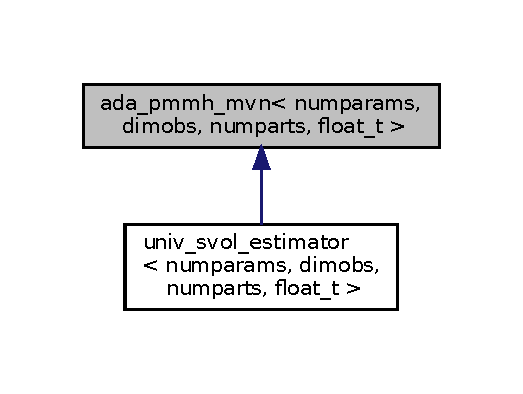
\includegraphics[width=251pt]{classada__pmmh__mvn__inherit__graph}
\end{center}
\end{figure}


Collaboration diagram for ada\+\_\+pmmh\+\_\+mvn$<$ numparams, dimobs, numparts, float\+\_\+t $>$\+:
\nopagebreak
\begin{figure}[H]
\begin{center}
\leavevmode
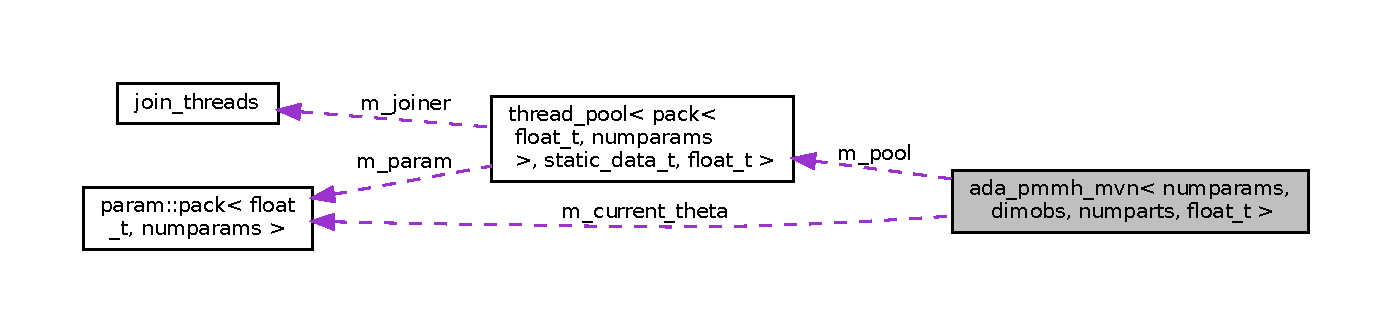
\includegraphics[width=350pt]{classada__pmmh__mvn__coll__graph}
\end{center}
\end{figure}
\doxysubsection*{Public Types}
\begin{DoxyCompactItemize}
\item 
\mbox{\Hypertarget{classada__pmmh__mvn_af036f732a29ede6fee08cdaacc9bbaaa}\label{classada__pmmh__mvn_af036f732a29ede6fee08cdaacc9bbaaa}} 
using {\bfseries osv} = Eigen\+::\+Matrix$<$ float\+\_\+t, dimobs, 1 $>$
\item 
\mbox{\Hypertarget{classada__pmmh__mvn_adb9df4d2086af9cace0f8aeebd805a73}\label{classada__pmmh__mvn_adb9df4d2086af9cace0f8aeebd805a73}} 
using {\bfseries psv} = Eigen\+::\+Matrix$<$ float\+\_\+t, numparams, 1 $>$
\item 
\mbox{\Hypertarget{classada__pmmh__mvn_a1cb69e6998319cbe2733965a177dc8d1}\label{classada__pmmh__mvn_a1cb69e6998319cbe2733965a177dc8d1}} 
using {\bfseries psm} = Eigen\+::\+Matrix$<$ float\+\_\+t, numparams, numparams $>$
\item 
\mbox{\Hypertarget{classada__pmmh__mvn_a49dd6f158687b02d8ea624f45a881f2e}\label{classada__pmmh__mvn_a49dd6f158687b02d8ea624f45a881f2e}} 
using {\bfseries dyn\+\_\+data\+\_\+t} = \mbox{\hyperlink{classparam_1_1pack}{param\+::pack}}$<$ float\+\_\+t, numparams $>$
\item 
\mbox{\Hypertarget{classada__pmmh__mvn_a0d8268928270a7f5d148d57655b250d1}\label{classada__pmmh__mvn_a0d8268928270a7f5d148d57655b250d1}} 
using {\bfseries static\+\_\+data\+\_\+t} = std\+::vector$<$ osv $>$
\end{DoxyCompactItemize}
\doxysubsection*{Public Member Functions}
\begin{DoxyCompactItemize}
\item 
\mbox{\hyperlink{classada__pmmh__mvn_a0caebfbc6ff008ac1fcca2a09c06d4a5}{ada\+\_\+pmmh\+\_\+mvn}} (const psv \&start\+\_\+trans\+\_\+theta, std\+::vector$<$ std\+::string $>$ tts, const unsigned int \&num\+\_\+mcmc\+\_\+iters, const unsigned int \&num\+\_\+pfilters, const std\+::string \&data\+\_\+file, const std\+::string \&sample\+\_\+file\+\_\+base\+\_\+name, const std\+::string \&message\+\_\+file\+\_\+base\+\_\+name, const bool \&mc, const unsigned int \&t0, const unsigned int \&t1, const psm \&C0, bool print\+\_\+to\+\_\+console, unsigned int print\+\_\+every\+\_\+k)
\begin{DoxyCompactList}\small\item\em Constructs algorithm object. \end{DoxyCompactList}\item 
psm \mbox{\hyperlink{classada__pmmh__mvn_a06930a79f4d2a62aa0cf24528c77e5a7}{get\+\_\+ct}} () const
\begin{DoxyCompactList}\small\item\em Get the current proposal distribution\textquotesingle{}s covariance matrix. \end{DoxyCompactList}\item 
\mbox{\Hypertarget{classada__pmmh__mvn_a60ddc5d58cb45d40aa455b6fe7aaa55e}\label{classada__pmmh__mvn_a60ddc5d58cb45d40aa455b6fe7aaa55e}} 
void \mbox{\hyperlink{classada__pmmh__mvn_a60ddc5d58cb45d40aa455b6fe7aaa55e}{commence\+\_\+sampling}} ()
\begin{DoxyCompactList}\small\item\em starts the sampling \end{DoxyCompactList}\item 
virtual float\+\_\+t \mbox{\hyperlink{classada__pmmh__mvn_a328bdc11578fac9397b4a2ee6cec5da2}{log\+\_\+prior\+\_\+eval}} (const \mbox{\hyperlink{classparam_1_1pack}{param\+::pack}}$<$ float\+\_\+t, numparams $>$ \&theta)=0
\begin{DoxyCompactList}\small\item\em Evaluates the log of the model\textquotesingle{}s prior. \end{DoxyCompactList}\item 
virtual float\+\_\+t \mbox{\hyperlink{classada__pmmh__mvn_a3f447b26c5adcbff9c7d2dfe46f5f59e}{log\+\_\+like\+\_\+eval}} (const \mbox{\hyperlink{classparam_1_1pack}{param\+::pack}}$<$ float\+\_\+t, numparams $>$ \&theta, const std\+::vector$<$ osv $>$ \&data)=0
\begin{DoxyCompactList}\small\item\em Evaluates (approximates) the log-\/likelihood with a particle filter. \end{DoxyCompactList}\end{DoxyCompactItemize}
\doxysubsection*{Private Member Functions}
\begin{DoxyCompactItemize}
\item 
\mbox{\Hypertarget{classada__pmmh__mvn_a5d2c0b95de487592cbd3a37a0d492a95}\label{classada__pmmh__mvn_a5d2c0b95de487592cbd3a37a0d492a95}} 
void {\bfseries update\+\_\+moments\+\_\+and\+\_\+\+Ct} (const \mbox{\hyperlink{classparam_1_1pack}{dyn\+\_\+data\+\_\+t}} \&new\+\_\+theta)
\item 
\mbox{\Hypertarget{classada__pmmh__mvn_a7feb6dc99c0be41e98291566b3e8beca}\label{classada__pmmh__mvn_a7feb6dc99c0be41e98291566b3e8beca}} 
psv {\bfseries q\+\_\+samp} (const \mbox{\hyperlink{classparam_1_1pack}{dyn\+\_\+data\+\_\+t}} \&old\+\_\+theta)
\item 
\mbox{\Hypertarget{classada__pmmh__mvn_a897aa2613645acffd64ffcfc920bc7cd}\label{classada__pmmh__mvn_a897aa2613645acffd64ffcfc920bc7cd}} 
float\+\_\+t {\bfseries log\+\_\+q\+\_\+eval} (const \mbox{\hyperlink{classparam_1_1pack}{dyn\+\_\+data\+\_\+t}} \&old\+Params, const \mbox{\hyperlink{classparam_1_1pack}{dyn\+\_\+data\+\_\+t}} \&new\+\_\+params)
\item 
\mbox{\Hypertarget{classada__pmmh__mvn_acc264e0934413d7d57be3cd0f22bb4c6}\label{classada__pmmh__mvn_acc264e0934413d7d57be3cd0f22bb4c6}} 
void {\bfseries record\+\_\+params} ()
\item 
\mbox{\Hypertarget{classada__pmmh__mvn_a40213871b135a68e35f0bc3536796f1f}\label{classada__pmmh__mvn_a40213871b135a68e35f0bc3536796f1f}} 
void {\bfseries record\+\_\+iter\+\_\+num} ()
\item 
\mbox{\Hypertarget{classada__pmmh__mvn_abc411ba7288980b0dbafc97b7286a62e}\label{classada__pmmh__mvn_abc411ba7288980b0dbafc97b7286a62e}} 
void {\bfseries record\+\_\+messages} ()
\item 
\mbox{\Hypertarget{classada__pmmh__mvn_a9a2fd1ae3f4a6c08b1ac54764c24d73e}\label{classada__pmmh__mvn_a9a2fd1ae3f4a6c08b1ac54764c24d73e}} 
float\+\_\+t {\bfseries pool\+\_\+func} (\mbox{\hyperlink{classparam_1_1pack}{dyn\+\_\+data\+\_\+t}} param, static\+\_\+data\+\_\+t obs\+\_\+data)
\item 
\mbox{\Hypertarget{classada__pmmh__mvn_afd3009731c19e2d634041c0a97bcaecb}\label{classada__pmmh__mvn_afd3009731c19e2d634041c0a97bcaecb}} 
std\+::string \mbox{\hyperlink{classada__pmmh__mvn_afd3009731c19e2d634041c0a97bcaecb}{gen\+\_\+string\+\_\+with\+\_\+time}} (const std\+::string \&str)
\begin{DoxyCompactList}\small\item\em return string with format is Y\+Y\+Y\+Y-\/\+M\+M-\/\+D\+D.\+HH\+:mm\+:ss \end{DoxyCompactList}\end{DoxyCompactItemize}
\doxysubsection*{Private Attributes}
\begin{DoxyCompactItemize}
\item 
\mbox{\Hypertarget{classada__pmmh__mvn_a963f9dac96b9c1f14cbc5bca91f629eb}\label{classada__pmmh__mvn_a963f9dac96b9c1f14cbc5bca91f629eb}} 
\mbox{\hyperlink{classparam_1_1pack}{dyn\+\_\+data\+\_\+t}} {\bfseries m\+\_\+current\+\_\+theta}
\item 
\mbox{\Hypertarget{classada__pmmh__mvn_a53ea30078083dcbe435ece00c7f5bc6e}\label{classada__pmmh__mvn_a53ea30078083dcbe435ece00c7f5bc6e}} 
std\+::vector$<$ std\+::string $>$ {\bfseries m\+\_\+tts}
\item 
\mbox{\Hypertarget{classada__pmmh__mvn_afff9cd2d50bb0577aa861f30df27d4eb}\label{classada__pmmh__mvn_afff9cd2d50bb0577aa861f30df27d4eb}} 
psm {\bfseries m\+\_\+sigma\+\_\+hat}
\item 
\mbox{\Hypertarget{classada__pmmh__mvn_ab95fb64336166bbad83562a75f80a1f7}\label{classada__pmmh__mvn_ab95fb64336166bbad83562a75f80a1f7}} 
psv {\bfseries m\+\_\+mean\+\_\+trans\+\_\+theta}
\item 
\mbox{\Hypertarget{classada__pmmh__mvn_a668c49d3ef53a5c69dcc96b4784a34f0}\label{classada__pmmh__mvn_a668c49d3ef53a5c69dcc96b4784a34f0}} 
float\+\_\+t {\bfseries m\+\_\+ma\+\_\+accept\+\_\+rate}
\item 
\mbox{\Hypertarget{classada__pmmh__mvn_aa8208a1108ef730a8f67efce9c804753}\label{classada__pmmh__mvn_aa8208a1108ef730a8f67efce9c804753}} 
unsigned int {\bfseries m\+\_\+t0}
\item 
\mbox{\Hypertarget{classada__pmmh__mvn_ab3cf6f22e3efd4869eca06c78325b20f}\label{classada__pmmh__mvn_ab3cf6f22e3efd4869eca06c78325b20f}} 
unsigned int {\bfseries m\+\_\+t1}
\item 
\mbox{\Hypertarget{classada__pmmh__mvn_a8b2d63854397e746b7118c75e310686b}\label{classada__pmmh__mvn_a8b2d63854397e746b7118c75e310686b}} 
psm {\bfseries m\+\_\+\+Ct}
\item 
\mbox{\Hypertarget{classada__pmmh__mvn_a0d49f77bf7ea14f780f6192ad520410f}\label{classada__pmmh__mvn_a0d49f77bf7ea14f780f6192ad520410f}} 
rvsamp\+::\+M\+V\+N\+Sampler$<$ numparams, float\+\_\+t $>$ {\bfseries m\+\_\+mvn\+\_\+gen}
\item 
\mbox{\Hypertarget{classada__pmmh__mvn_aa2f05575406feb4bc2e7ed97d9edb703}\label{classada__pmmh__mvn_aa2f05575406feb4bc2e7ed97d9edb703}} 
std\+::ofstream {\bfseries m\+\_\+samples\+\_\+file\+\_\+stream}
\item 
\mbox{\Hypertarget{classada__pmmh__mvn_ad04a7bd0a0cf81836cbc3934b2b40ece}\label{classada__pmmh__mvn_ad04a7bd0a0cf81836cbc3934b2b40ece}} 
std\+::ofstream {\bfseries m\+\_\+message\+\_\+stream}
\item 
\mbox{\Hypertarget{classada__pmmh__mvn_a653603682a96d0f30c82f5f5bd83503e}\label{classada__pmmh__mvn_a653603682a96d0f30c82f5f5bd83503e}} 
unsigned int {\bfseries m\+\_\+num\+\_\+mcmc\+\_\+iters}
\item 
\mbox{\Hypertarget{classada__pmmh__mvn_a06b5eed1ebb523262ec69e46bc70393d}\label{classada__pmmh__mvn_a06b5eed1ebb523262ec69e46bc70393d}} 
unsigned int {\bfseries m\+\_\+iter}
\item 
\mbox{\Hypertarget{classada__pmmh__mvn_ad33ac891e9fb4bd9b59185d874d05301}\label{classada__pmmh__mvn_ad33ac891e9fb4bd9b59185d874d05301}} 
float\+\_\+t {\bfseries m\+\_\+sd}
\item 
\mbox{\Hypertarget{classada__pmmh__mvn_abaf7185b58d25568b0032903e5fc1748}\label{classada__pmmh__mvn_abaf7185b58d25568b0032903e5fc1748}} 
float\+\_\+t {\bfseries m\+\_\+eps}
\item 
\mbox{\Hypertarget{classada__pmmh__mvn_a9f1b4d3880798e8f0d72728f51fbaf32}\label{classada__pmmh__mvn_a9f1b4d3880798e8f0d72728f51fbaf32}} 
bool {\bfseries m\+\_\+print\+\_\+to\+\_\+console}
\item 
\mbox{\Hypertarget{classada__pmmh__mvn_ab1eb75f119d61924cdbfa9b00c07d795}\label{classada__pmmh__mvn_ab1eb75f119d61924cdbfa9b00c07d795}} 
unsigned int {\bfseries m\+\_\+print\+\_\+every\+\_\+k}
\item 
\mbox{\Hypertarget{classada__pmmh__mvn_a61d44e7e37a40c78fe93731a5f85e36a}\label{classada__pmmh__mvn_a61d44e7e37a40c78fe93731a5f85e36a}} 
\mbox{\hyperlink{classthread__pool}{thread\+\_\+pool}}$<$ \mbox{\hyperlink{classparam_1_1pack}{dyn\+\_\+data\+\_\+t}}, static\+\_\+data\+\_\+t, float\+\_\+t $>$ {\bfseries m\+\_\+pool}
\item 
\mbox{\Hypertarget{classada__pmmh__mvn_aef282ba683044bc137b97fb5b77938eb}\label{classada__pmmh__mvn_aef282ba683044bc137b97fb5b77938eb}} 
float\+\_\+t {\bfseries m\+\_\+old\+\_\+log\+\_\+like}
\item 
\mbox{\Hypertarget{classada__pmmh__mvn_a7efb1aa460765803a0b1655e5513e5b5}\label{classada__pmmh__mvn_a7efb1aa460765803a0b1655e5513e5b5}} 
float\+\_\+t {\bfseries m\+\_\+new\+\_\+log\+\_\+like}
\item 
\mbox{\Hypertarget{classada__pmmh__mvn_add751ce82e67547ad92762b613894da3}\label{classada__pmmh__mvn_add751ce82e67547ad92762b613894da3}} 
float\+\_\+t {\bfseries m\+\_\+old\+\_\+log\+\_\+prior}
\item 
\mbox{\Hypertarget{classada__pmmh__mvn_a64d5bec4b3083b64e592bd14fb56d3f1}\label{classada__pmmh__mvn_a64d5bec4b3083b64e592bd14fb56d3f1}} 
float\+\_\+t {\bfseries m\+\_\+new\+\_\+log\+\_\+prior}
\item 
\mbox{\Hypertarget{classada__pmmh__mvn_a9f5e52f06042c58757d87cb8745e6bf3}\label{classada__pmmh__mvn_a9f5e52f06042c58757d87cb8745e6bf3}} 
float\+\_\+t {\bfseries m\+\_\+log\+\_\+accept\+\_\+prob}
\item 
\mbox{\Hypertarget{classada__pmmh__mvn_a526172f6b05745044b469f669aa26660}\label{classada__pmmh__mvn_a526172f6b05745044b469f669aa26660}} 
bool {\bfseries m\+\_\+accepted}
\end{DoxyCompactItemize}


\doxysubsection{Detailed Description}
\subsubsection*{template$<$size\+\_\+t numparams, size\+\_\+t dimobs, size\+\_\+t numparts, typename float\+\_\+t$>$\newline
class ada\+\_\+pmmh\+\_\+mvn$<$ numparams, dimobs, numparts, float\+\_\+t $>$}

\begin{DoxyAuthor}{Author}
Taylor 
\end{DoxyAuthor}


\doxysubsection{Constructor \& Destructor Documentation}
\mbox{\Hypertarget{classada__pmmh__mvn_a0caebfbc6ff008ac1fcca2a09c06d4a5}\label{classada__pmmh__mvn_a0caebfbc6ff008ac1fcca2a09c06d4a5}} 
\index{ada\_pmmh\_mvn$<$ numparams, dimobs, numparts, float\_t $>$@{ada\_pmmh\_mvn$<$ numparams, dimobs, numparts, float\_t $>$}!ada\_pmmh\_mvn@{ada\_pmmh\_mvn}}
\index{ada\_pmmh\_mvn@{ada\_pmmh\_mvn}!ada\_pmmh\_mvn$<$ numparams, dimobs, numparts, float\_t $>$@{ada\_pmmh\_mvn$<$ numparams, dimobs, numparts, float\_t $>$}}
\doxysubsubsection{\texorpdfstring{ada\_pmmh\_mvn()}{ada\_pmmh\_mvn()}}
{\footnotesize\ttfamily template$<$size\+\_\+t numparams, size\+\_\+t dimobs, size\+\_\+t numparts, typename float\+\_\+t $>$ \\
\mbox{\hyperlink{classada__pmmh__mvn}{ada\+\_\+pmmh\+\_\+mvn}}$<$ numparams, dimobs, numparts, float\+\_\+t $>$\+::\mbox{\hyperlink{classada__pmmh__mvn}{ada\+\_\+pmmh\+\_\+mvn}} (\begin{DoxyParamCaption}\item[{const psv \&}]{start\+\_\+trans\+\_\+theta,  }\item[{std\+::vector$<$ std\+::string $>$}]{tts,  }\item[{const unsigned int \&}]{num\+\_\+mcmc\+\_\+iters,  }\item[{const unsigned int \&}]{num\+\_\+pfilters,  }\item[{const std\+::string \&}]{data\+\_\+file,  }\item[{const std\+::string \&}]{sample\+\_\+file\+\_\+base\+\_\+name,  }\item[{const std\+::string \&}]{message\+\_\+file\+\_\+base\+\_\+name,  }\item[{const bool \&}]{mc,  }\item[{const unsigned int \&}]{t0,  }\item[{const unsigned int \&}]{t1,  }\item[{const psm \&}]{C0,  }\item[{bool}]{print\+\_\+to\+\_\+console,  }\item[{unsigned int}]{print\+\_\+every\+\_\+k }\end{DoxyParamCaption})}



Constructs algorithm object. 


\begin{DoxyParams}{Parameters}
{\em start\+\_\+trans\+\_\+theta} & the initial transformed parameters you want to start sampling from. \\
\hline
{\em num\+\_\+mcmc\+\_\+iters} & the number of M\+C\+MC iterations you want to do. \\
\hline
{\em data\+\_\+file} & the location of the observed time series data (input). \\
\hline
{\em samples\+\_\+file} & the location where you want to store the theta samples (output). \\
\hline
{\em messages\+\_\+file} & the location where you want to store the messages (output). \\
\hline
{\em mc} & stands for multicore. true or false if you want to use extra cores. \\
\hline
{\em t0} & iteration you start adapting \\
\hline
{\em t1} & iteration you stop adapting \\
\hline
{\em C0} & initial covariance matrix for proposal distribution. \\
\hline
{\em print\+\_\+to\+\_\+console} & true if you want to see messages in real time \\
\hline
{\em print\+\_\+every\+\_\+k} & print messages and samples every (this number) iterations \\
\hline
\end{DoxyParams}


\doxysubsection{Member Function Documentation}
\mbox{\Hypertarget{classada__pmmh__mvn_a06930a79f4d2a62aa0cf24528c77e5a7}\label{classada__pmmh__mvn_a06930a79f4d2a62aa0cf24528c77e5a7}} 
\index{ada\_pmmh\_mvn$<$ numparams, dimobs, numparts, float\_t $>$@{ada\_pmmh\_mvn$<$ numparams, dimobs, numparts, float\_t $>$}!get\_ct@{get\_ct}}
\index{get\_ct@{get\_ct}!ada\_pmmh\_mvn$<$ numparams, dimobs, numparts, float\_t $>$@{ada\_pmmh\_mvn$<$ numparams, dimobs, numparts, float\_t $>$}}
\doxysubsubsection{\texorpdfstring{get\_ct()}{get\_ct()}}
{\footnotesize\ttfamily template$<$size\+\_\+t numparams, size\+\_\+t dimobs, size\+\_\+t numparts, typename float\+\_\+t $>$ \\
auto \mbox{\hyperlink{classada__pmmh__mvn}{ada\+\_\+pmmh\+\_\+mvn}}$<$ numparams, dimobs, numparts, float\+\_\+t $>$\+::get\+\_\+ct}



Get the current proposal distribution\textquotesingle{}s covariance matrix. 

\begin{DoxyReturn}{Returns}
the covariance matrix of q(theta\textquotesingle{} $\vert$ theta) 
\end{DoxyReturn}
\mbox{\Hypertarget{classada__pmmh__mvn_a3f447b26c5adcbff9c7d2dfe46f5f59e}\label{classada__pmmh__mvn_a3f447b26c5adcbff9c7d2dfe46f5f59e}} 
\index{ada\_pmmh\_mvn$<$ numparams, dimobs, numparts, float\_t $>$@{ada\_pmmh\_mvn$<$ numparams, dimobs, numparts, float\_t $>$}!log\_like\_eval@{log\_like\_eval}}
\index{log\_like\_eval@{log\_like\_eval}!ada\_pmmh\_mvn$<$ numparams, dimobs, numparts, float\_t $>$@{ada\_pmmh\_mvn$<$ numparams, dimobs, numparts, float\_t $>$}}
\doxysubsubsection{\texorpdfstring{log\_like\_eval()}{log\_like\_eval()}}
{\footnotesize\ttfamily template$<$size\+\_\+t numparams, size\+\_\+t dimobs, size\+\_\+t numparts, typename float\+\_\+t $>$ \\
virtual float\+\_\+t \mbox{\hyperlink{classada__pmmh__mvn}{ada\+\_\+pmmh\+\_\+mvn}}$<$ numparams, dimobs, numparts, float\+\_\+t $>$\+::log\+\_\+like\+\_\+eval (\begin{DoxyParamCaption}\item[{const \mbox{\hyperlink{classparam_1_1pack}{param\+::pack}}$<$ float\+\_\+t, numparams $>$ \&}]{theta,  }\item[{const std\+::vector$<$ osv $>$ \&}]{data }\end{DoxyParamCaption})\hspace{0.3cm}{\ttfamily [pure virtual]}}



Evaluates (approximates) the log-\/likelihood with a particle filter. 


\begin{DoxyParams}{Parameters}
{\em theta} & the parameters with which to run the particle filter \\
\hline
{\em data} & the observed data with which to run the particle filter \\
\hline
\end{DoxyParams}
\begin{DoxyReturn}{Returns}
the evaluation of the approx. log likelihood 
\end{DoxyReturn}
\mbox{\Hypertarget{classada__pmmh__mvn_a328bdc11578fac9397b4a2ee6cec5da2}\label{classada__pmmh__mvn_a328bdc11578fac9397b4a2ee6cec5da2}} 
\index{ada\_pmmh\_mvn$<$ numparams, dimobs, numparts, float\_t $>$@{ada\_pmmh\_mvn$<$ numparams, dimobs, numparts, float\_t $>$}!log\_prior\_eval@{log\_prior\_eval}}
\index{log\_prior\_eval@{log\_prior\_eval}!ada\_pmmh\_mvn$<$ numparams, dimobs, numparts, float\_t $>$@{ada\_pmmh\_mvn$<$ numparams, dimobs, numparts, float\_t $>$}}
\doxysubsubsection{\texorpdfstring{log\_prior\_eval()}{log\_prior\_eval()}}
{\footnotesize\ttfamily template$<$size\+\_\+t numparams, size\+\_\+t dimobs, size\+\_\+t numparts, typename float\+\_\+t $>$ \\
virtual float\+\_\+t \mbox{\hyperlink{classada__pmmh__mvn}{ada\+\_\+pmmh\+\_\+mvn}}$<$ numparams, dimobs, numparts, float\+\_\+t $>$\+::log\+\_\+prior\+\_\+eval (\begin{DoxyParamCaption}\item[{const \mbox{\hyperlink{classparam_1_1pack}{param\+::pack}}$<$ float\+\_\+t, numparams $>$ \&}]{theta }\end{DoxyParamCaption})\hspace{0.3cm}{\ttfamily [pure virtual]}}



Evaluates the log of the model\textquotesingle{}s prior. 


\begin{DoxyParams}{Parameters}
{\em theta} & the parameters argument \\
\hline
\end{DoxyParams}
\begin{DoxyReturn}{Returns}
the log of the prior density 
\end{DoxyReturn}


The documentation for this class was generated from the following file\+:\begin{DoxyCompactItemize}
\item 
include/ssme/\mbox{\hyperlink{ada__pmmh__mvn_8h}{ada\+\_\+pmmh\+\_\+mvn.\+h}}\end{DoxyCompactItemize}

\hypertarget{classada__rwmh}{}\section{ada\+\_\+rwmh$<$ numparams, dimobs, float\+\_\+t $>$ Class Template Reference}
\label{classada__rwmh}\index{ada\+\_\+rwmh$<$ numparams, dimobs, float\+\_\+t $>$@{ada\+\_\+rwmh$<$ numparams, dimobs, float\+\_\+t $>$}}


{\ttfamily \#include $<$ada\+\_\+rwmh.\+h$>$}

\subsection*{Public Types}
\begin{DoxyCompactItemize}
\item 
\mbox{\Hypertarget{classada__rwmh_aeb76bd00a699bb238958637c862c1056}\label{classada__rwmh_aeb76bd00a699bb238958637c862c1056}} 
using {\bfseries osv} = Eigen\+::\+Matrix$<$ float\+\_\+t, dimobs, 1 $>$
\item 
\mbox{\Hypertarget{classada__rwmh_aac7b75115f3e74764d44cb845bd17208}\label{classada__rwmh_aac7b75115f3e74764d44cb845bd17208}} 
using {\bfseries psv} = Eigen\+::\+Matrix$<$ float\+\_\+t, numparams, 1 $>$
\item 
\mbox{\Hypertarget{classada__rwmh_a8259b89462a9f732bd8a6792a84903be}\label{classada__rwmh_a8259b89462a9f732bd8a6792a84903be}} 
using {\bfseries psm} = Eigen\+::\+Matrix$<$ float\+\_\+t, numparams, numparams $>$
\end{DoxyCompactItemize}
\subsection*{Public Member Functions}
\begin{DoxyCompactItemize}
\item 
\hyperlink{classada__rwmh_a6bf39cdf5a3a5aec9baa3018364131d6}{ada\+\_\+rwmh} (const psv \&start\+\_\+trans\+\_\+theta, const std\+::vector$<$ \hyperlink{param__transforms_8h_acee593b112f4fc85f850631b9c6aaae9}{Trans\+Type} $>$ \&tts, const unsigned int \&num\+\_\+mcmc\+\_\+iters, const std\+::string \&data\+\_\+file, const std\+::string \&sample\+\_\+file\+\_\+base\+\_\+name, const std\+::string \&message\+\_\+file\+\_\+base\+\_\+name, const unsigned int \&t0, const unsigned int \&t1, const psm \&C0, bool print\+\_\+to\+\_\+console, unsigned int print\+\_\+every\+\_\+k)
\begin{DoxyCompactList}\small\item\em The constructor. \end{DoxyCompactList}\item 
psm \hyperlink{classada__rwmh_a72d5898fe897cba162456f269f385ade}{get\+\_\+ct} () const
\begin{DoxyCompactList}\small\item\em Get the current proposal distribution\textquotesingle{}s covariance matrix. \end{DoxyCompactList}\item 
void \hyperlink{classada__rwmh_a5f7905f68c0b07541fa1729304f8988f}{commence\+Sampling} (const std\+::vector$<$ Eigen\+::\+Matrix$<$ float\+\_\+t, dimobs, 1 $>$$>$ \&data)
\begin{DoxyCompactList}\small\item\em starts the sampling \end{DoxyCompactList}\item 
virtual float\+\_\+t \hyperlink{classada__rwmh_a859004bc1e241d55fbb3f072cf43d994}{log\+Prior\+Evaluate} (const \hyperlink{classparamPack}{param\+Pack}$<$ float\+\_\+t $>$ \&theta)=0
\begin{DoxyCompactList}\small\item\em Evaluates the log of the model\textquotesingle{}s prior distribution assuming the original/nontransformed/contrained parameterization. \end{DoxyCompactList}\item 
virtual float\+\_\+t \hyperlink{classada__rwmh_a403b60eaee01171bf05a7c73b53ac28f}{log\+Like\+Evaluate} (const \hyperlink{classparamPack}{param\+Pack}$<$ float\+\_\+t $>$ \&theta, const std\+::vector$<$ osv $>$ \&data)=0
\begin{DoxyCompactList}\small\item\em Evaluates the log-\/likelihood. \end{DoxyCompactList}\end{DoxyCompactItemize}
\subsection*{Private Member Functions}
\begin{DoxyCompactItemize}
\item 
\mbox{\Hypertarget{classada__rwmh_a42bb58088d56546dac06c2bd0aebda64}\label{classada__rwmh_a42bb58088d56546dac06c2bd0aebda64}} 
void {\bfseries update\+\_\+moments\+\_\+and\+\_\+\+Ct} (const \hyperlink{classparamPack}{param\+Pack}$<$ float\+\_\+t $>$ \&new\+Theta)
\item 
\mbox{\Hypertarget{classada__rwmh_a765ac73a9cf28f6847e0244149494253}\label{classada__rwmh_a765ac73a9cf28f6847e0244149494253}} 
psv {\bfseries q\+Sample} (const \hyperlink{classparamPack}{param\+Pack}$<$ float\+\_\+t $>$ \&old\+Theta)
\item 
\mbox{\Hypertarget{classada__rwmh_a429aaa769c48191d00ef00d69af803d3}\label{classada__rwmh_a429aaa769c48191d00ef00d69af803d3}} 
float\+\_\+t {\bfseries log\+Q\+Evaluate} (const \hyperlink{classparamPack}{param\+Pack}$<$ float\+\_\+t $>$ \&old\+Params, const \hyperlink{classparamPack}{param\+Pack}$<$ float\+\_\+t $>$ \&new\+Params)
\end{DoxyCompactItemize}
\subsection*{Private Attributes}
\begin{DoxyCompactItemize}
\item 
\mbox{\Hypertarget{classada__rwmh_a1640d72a3c8527ec1f8e852bb3528478}\label{classada__rwmh_a1640d72a3c8527ec1f8e852bb3528478}} 
\hyperlink{classparamPack}{param\+Pack}$<$ float\+\_\+t $>$ {\bfseries m\+\_\+current\+\_\+theta}
\item 
\mbox{\Hypertarget{classada__rwmh_ae482d387ff42e61bb2b639e7b9adcf1f}\label{classada__rwmh_ae482d387ff42e61bb2b639e7b9adcf1f}} 
std\+::vector$<$ \hyperlink{param__transforms_8h_acee593b112f4fc85f850631b9c6aaae9}{Trans\+Type} $>$ {\bfseries m\+\_\+tts}
\item 
\mbox{\Hypertarget{classada__rwmh_a8a33cccbf4a3f3f79d2c5648b7ed6ade}\label{classada__rwmh_a8a33cccbf4a3f3f79d2c5648b7ed6ade}} 
psm {\bfseries m\+\_\+sigma\+\_\+hat}
\item 
\mbox{\Hypertarget{classada__rwmh_ac0c5ef385c8e92458701f8a24536226b}\label{classada__rwmh_ac0c5ef385c8e92458701f8a24536226b}} 
psv {\bfseries m\+\_\+mean\+\_\+trans\+\_\+theta}
\item 
\mbox{\Hypertarget{classada__rwmh_ada2efc6c92c36f576cf82aab7f6b4edf}\label{classada__rwmh_ada2efc6c92c36f576cf82aab7f6b4edf}} 
float\+\_\+t {\bfseries m\+\_\+ma\+\_\+accept\+\_\+rate}
\item 
\mbox{\Hypertarget{classada__rwmh_a1cc1c6f7354098826cca89d2be20f26d}\label{classada__rwmh_a1cc1c6f7354098826cca89d2be20f26d}} 
unsigned int {\bfseries m\+\_\+t0}
\item 
\mbox{\Hypertarget{classada__rwmh_a4eb4ddfc05f7268ebeb94becf7e97479}\label{classada__rwmh_a4eb4ddfc05f7268ebeb94becf7e97479}} 
unsigned int {\bfseries m\+\_\+t1}
\item 
\mbox{\Hypertarget{classada__rwmh_a444fd1fd9a89d1cfe65a91d5c3f78804}\label{classada__rwmh_a444fd1fd9a89d1cfe65a91d5c3f78804}} 
psm {\bfseries m\+\_\+\+Ct}
\item 
\mbox{\Hypertarget{classada__rwmh_abefded0f465feca0978c62a23272f6e7}\label{classada__rwmh_abefded0f465feca0978c62a23272f6e7}} 
rvsamp\+::\+M\+V\+N\+Sampler$<$ numparams $>$ {\bfseries m\+\_\+mvn\+\_\+gen}
\item 
\mbox{\Hypertarget{classada__rwmh_a69dacf852ca273699f0feeb01eede483}\label{classada__rwmh_a69dacf852ca273699f0feeb01eede483}} 
std\+::ofstream {\bfseries m\+\_\+samples\+\_\+file\+\_\+stream}
\item 
\mbox{\Hypertarget{classada__rwmh_a7f8ad3832457b6cf2db86209f1d0815d}\label{classada__rwmh_a7f8ad3832457b6cf2db86209f1d0815d}} 
std\+::ofstream {\bfseries m\+\_\+message\+\_\+stream}
\item 
\mbox{\Hypertarget{classada__rwmh_a2185c88558348b04248284435ef33aed}\label{classada__rwmh_a2185c88558348b04248284435ef33aed}} 
unsigned int {\bfseries m\+\_\+num\+\_\+mcmc\+\_\+iters}
\item 
\mbox{\Hypertarget{classada__rwmh_a26cc21e17b8aa2eecb780dcbdd2bbf8a}\label{classada__rwmh_a26cc21e17b8aa2eecb780dcbdd2bbf8a}} 
unsigned int {\bfseries m\+\_\+iter}
\item 
\mbox{\Hypertarget{classada__rwmh_a4a595db36214f8cc05d131e705a7a508}\label{classada__rwmh_a4a595db36214f8cc05d131e705a7a508}} 
float\+\_\+t {\bfseries m\+\_\+sd}
\item 
\mbox{\Hypertarget{classada__rwmh_ab489b16e306c62dc58c225c64e1b9ee7}\label{classada__rwmh_ab489b16e306c62dc58c225c64e1b9ee7}} 
float\+\_\+t {\bfseries m\+\_\+eps}
\item 
\mbox{\Hypertarget{classada__rwmh_ae62e97c4a6916f1d6b3c70bd8a9fa176}\label{classada__rwmh_ae62e97c4a6916f1d6b3c70bd8a9fa176}} 
bool {\bfseries m\+\_\+print\+\_\+to\+\_\+console}
\item 
\mbox{\Hypertarget{classada__rwmh_ad919646e11969c8bc93360b88c8a3884}\label{classada__rwmh_ad919646e11969c8bc93360b88c8a3884}} 
unsigned int {\bfseries m\+\_\+print\+\_\+every\+\_\+k}
\end{DoxyCompactItemize}


\subsection{Detailed Description}
\subsubsection*{template$<$size\+\_\+t numparams, size\+\_\+t dimobs, typename float\+\_\+t$>$\newline
class ada\+\_\+rwmh$<$ numparams, dimobs, float\+\_\+t $>$}

\begin{DoxyAuthor}{Author}
t 
\end{DoxyAuthor}


\subsection{Constructor \& Destructor Documentation}
\mbox{\Hypertarget{classada__rwmh_a6bf39cdf5a3a5aec9baa3018364131d6}\label{classada__rwmh_a6bf39cdf5a3a5aec9baa3018364131d6}} 
\index{ada\+\_\+rwmh@{ada\+\_\+rwmh}!ada\+\_\+rwmh@{ada\+\_\+rwmh}}
\index{ada\+\_\+rwmh@{ada\+\_\+rwmh}!ada\+\_\+rwmh@{ada\+\_\+rwmh}}
\subsubsection{\texorpdfstring{ada\+\_\+rwmh()}{ada\_rwmh()}}
{\footnotesize\ttfamily template$<$size\+\_\+t numparams, size\+\_\+t dimobs, typename float\+\_\+t $>$ \\
\hyperlink{classada__rwmh}{ada\+\_\+rwmh}$<$ numparams, dimobs, float\+\_\+t $>$\+::\hyperlink{classada__rwmh}{ada\+\_\+rwmh} (\begin{DoxyParamCaption}\item[{const psv \&}]{start\+\_\+trans\+\_\+theta,  }\item[{const std\+::vector$<$ \hyperlink{param__transforms_8h_acee593b112f4fc85f850631b9c6aaae9}{Trans\+Type} $>$ \&}]{tts,  }\item[{const unsigned int \&}]{num\+\_\+mcmc\+\_\+iters,  }\item[{const std\+::string \&}]{data\+\_\+file,  }\item[{const std\+::string \&}]{sample\+\_\+file\+\_\+base\+\_\+name,  }\item[{const std\+::string \&}]{message\+\_\+file\+\_\+base\+\_\+name,  }\item[{const unsigned int \&}]{t0,  }\item[{const unsigned int \&}]{t1,  }\item[{const psm \&}]{C0,  }\item[{bool}]{print\+\_\+to\+\_\+console,  }\item[{unsigned int}]{print\+\_\+every\+\_\+k }\end{DoxyParamCaption})}



The constructor. 


\begin{DoxyParams}{Parameters}
{\em start\+\_\+trans\+\_\+theta} & the initial transformed parameters you want to start sampling from. \\
\hline
{\em num\+\_\+mcmc\+\_\+iters} & the number of M\+C\+MC iterations you want to do. \\
\hline
{\em data\+\_\+file} & the location of the observed time series data (input). \\
\hline
{\em samples\+\_\+file} & the location where you want to store the theta samples (output). \\
\hline
{\em messages\+\_\+file} & the location where you want to store the messages (output). \\
\hline
{\em t0} & time you start adapting \\
\hline
{\em t1} & time you stop adapting \\
\hline
{\em C0} & initial covariance matrix for proposal distribution. \\
\hline
{\em print\+\_\+to\+\_\+console} & true if you want to print messages to console (slow!) \\
\hline
{\em print\+\_\+every\+\_\+k} & (must be greater than 0, applies to logging parameters as well as writing out messages) \\
\hline
\end{DoxyParams}


\subsection{Member Function Documentation}
\mbox{\Hypertarget{classada__rwmh_a5f7905f68c0b07541fa1729304f8988f}\label{classada__rwmh_a5f7905f68c0b07541fa1729304f8988f}} 
\index{ada\+\_\+rwmh@{ada\+\_\+rwmh}!commence\+Sampling@{commence\+Sampling}}
\index{commence\+Sampling@{commence\+Sampling}!ada\+\_\+rwmh@{ada\+\_\+rwmh}}
\subsubsection{\texorpdfstring{commence\+Sampling()}{commenceSampling()}}
{\footnotesize\ttfamily template$<$size\+\_\+t numparams, size\+\_\+t dimobs, typename float\+\_\+t $>$ \\
void \hyperlink{classada__rwmh}{ada\+\_\+rwmh}$<$ numparams, dimobs, float\+\_\+t $>$\+::commence\+Sampling (\begin{DoxyParamCaption}\item[{const std\+::vector$<$ Eigen\+::\+Matrix$<$ float\+\_\+t, dimobs, 1 $>$$>$ \&}]{data }\end{DoxyParamCaption})}



starts the sampling 

!!!!! \mbox{\Hypertarget{classada__rwmh_a72d5898fe897cba162456f269f385ade}\label{classada__rwmh_a72d5898fe897cba162456f269f385ade}} 
\index{ada\+\_\+rwmh@{ada\+\_\+rwmh}!get\+\_\+ct@{get\+\_\+ct}}
\index{get\+\_\+ct@{get\+\_\+ct}!ada\+\_\+rwmh@{ada\+\_\+rwmh}}
\subsubsection{\texorpdfstring{get\+\_\+ct()}{get\_ct()}}
{\footnotesize\ttfamily template$<$size\+\_\+t numparams, size\+\_\+t dimobs, typename float\+\_\+t $>$ \\
auto \hyperlink{classada__rwmh}{ada\+\_\+rwmh}$<$ numparams, dimobs, float\+\_\+t $>$\+::get\+\_\+ct (\begin{DoxyParamCaption}{ }\end{DoxyParamCaption}) const}



Get the current proposal distribution\textquotesingle{}s covariance matrix. 

\begin{DoxyReturn}{Returns}
the covariance matrix of q(theta\textquotesingle{} $\vert$ theta) 
\end{DoxyReturn}
\mbox{\Hypertarget{classada__rwmh_a403b60eaee01171bf05a7c73b53ac28f}\label{classada__rwmh_a403b60eaee01171bf05a7c73b53ac28f}} 
\index{ada\+\_\+rwmh@{ada\+\_\+rwmh}!log\+Like\+Evaluate@{log\+Like\+Evaluate}}
\index{log\+Like\+Evaluate@{log\+Like\+Evaluate}!ada\+\_\+rwmh@{ada\+\_\+rwmh}}
\subsubsection{\texorpdfstring{log\+Like\+Evaluate()}{logLikeEvaluate()}}
{\footnotesize\ttfamily template$<$size\+\_\+t numparams, size\+\_\+t dimobs, typename float\+\_\+t $>$ \\
virtual float\+\_\+t \hyperlink{classada__rwmh}{ada\+\_\+rwmh}$<$ numparams, dimobs, float\+\_\+t $>$\+::log\+Like\+Evaluate (\begin{DoxyParamCaption}\item[{const \hyperlink{classparamPack}{param\+Pack}$<$ float\+\_\+t $>$ \&}]{theta,  }\item[{const std\+::vector$<$ osv $>$ \&}]{data }\end{DoxyParamCaption})\hspace{0.3cm}{\ttfamily [pure virtual]}}



Evaluates the log-\/likelihood. 


\begin{DoxyParams}{Parameters}
{\em theta} & the parameters of your likelihood. \\
\hline
{\em data} & the observed data you\textquotesingle{}re modeling. \\
\hline
\end{DoxyParams}
\begin{DoxyReturn}{Returns}
the evaluation (as a float\+\_\+t) of the log likelihood. 
\end{DoxyReturn}
\mbox{\Hypertarget{classada__rwmh_a859004bc1e241d55fbb3f072cf43d994}\label{classada__rwmh_a859004bc1e241d55fbb3f072cf43d994}} 
\index{ada\+\_\+rwmh@{ada\+\_\+rwmh}!log\+Prior\+Evaluate@{log\+Prior\+Evaluate}}
\index{log\+Prior\+Evaluate@{log\+Prior\+Evaluate}!ada\+\_\+rwmh@{ada\+\_\+rwmh}}
\subsubsection{\texorpdfstring{log\+Prior\+Evaluate()}{logPriorEvaluate()}}
{\footnotesize\ttfamily template$<$size\+\_\+t numparams, size\+\_\+t dimobs, typename float\+\_\+t $>$ \\
virtual float\+\_\+t \hyperlink{classada__rwmh}{ada\+\_\+rwmh}$<$ numparams, dimobs, float\+\_\+t $>$\+::log\+Prior\+Evaluate (\begin{DoxyParamCaption}\item[{const \hyperlink{classparamPack}{param\+Pack}$<$ float\+\_\+t $>$ \&}]{theta }\end{DoxyParamCaption})\hspace{0.3cm}{\ttfamily [pure virtual]}}



Evaluates the log of the model\textquotesingle{}s prior distribution assuming the original/nontransformed/contrained parameterization. 


\begin{DoxyParams}{Parameters}
{\em theta} & the parameters argument (nontransformed/constrained parameterization). \\
\hline
\end{DoxyParams}
\begin{DoxyReturn}{Returns}
the log of the prior density. 
\end{DoxyReturn}


The documentation for this class was generated from the following file\+:\begin{DoxyCompactItemize}
\item 
include/\hyperlink{ada__rwmh_8h}{ada\+\_\+rwmh.\+h}\end{DoxyCompactItemize}

\hypertarget{classlogitTrans}{}\section{logit\+Trans$<$ float\+\_\+t $>$ Class Template Reference}
\label{classlogitTrans}\index{logit\+Trans$<$ float\+\_\+t $>$@{logit\+Trans$<$ float\+\_\+t $>$}}


{\ttfamily \#include $<$param\+\_\+transforms.\+h$>$}



Inheritance diagram for logit\+Trans$<$ float\+\_\+t $>$\+:
\nopagebreak
\begin{figure}[H]
\begin{center}
\leavevmode
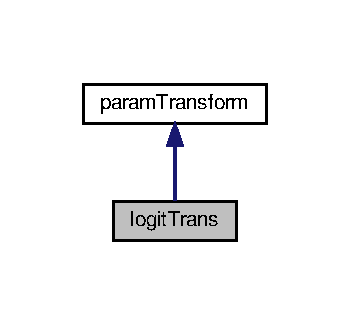
\includegraphics[width=213pt]{classlogitTrans__inherit__graph}
\end{center}
\end{figure}


Collaboration diagram for logit\+Trans$<$ float\+\_\+t $>$\+:
\nopagebreak
\begin{figure}[H]
\begin{center}
\leavevmode
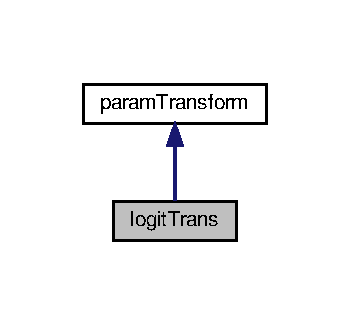
\includegraphics[width=213pt]{classlogitTrans__coll__graph}
\end{center}
\end{figure}
\subsection*{Public Member Functions}
\begin{DoxyCompactItemize}
\item 
\mbox{\Hypertarget{classlogitTrans_aee8d4c1429bebe62aefb64f07f88d8e0}\label{classlogitTrans_aee8d4c1429bebe62aefb64f07f88d8e0}} 
float\+\_\+t \hyperlink{classlogitTrans_aee8d4c1429bebe62aefb64f07f88d8e0}{trans} (const float\+\_\+t \&p) override
\begin{DoxyCompactList}\small\item\em from the constrained/nontransformed to the transformed/unconstrained space \end{DoxyCompactList}\item 
\mbox{\Hypertarget{classlogitTrans_ae0211473231a08e0a6feb54301ba8e45}\label{classlogitTrans_ae0211473231a08e0a6feb54301ba8e45}} 
float\+\_\+t \hyperlink{classlogitTrans_ae0211473231a08e0a6feb54301ba8e45}{inv\+Trans} (const float\+\_\+t \&trans\+\_\+p) override
\begin{DoxyCompactList}\small\item\em from the unconstrained/transformed to the constrained/untransformed space; \end{DoxyCompactList}\item 
\mbox{\Hypertarget{classlogitTrans_aef153d5f930c7c96e6f12c0def6220d9}\label{classlogitTrans_aef153d5f930c7c96e6f12c0def6220d9}} 
float\+\_\+t \hyperlink{classlogitTrans_aef153d5f930c7c96e6f12c0def6220d9}{log\+Jacobian} (const float\+\_\+t \&p) override
\begin{DoxyCompactList}\small\item\em get the log jacobian (from untransformed to transformed). For use with adjusting priors to the transformed space. \end{DoxyCompactList}\end{DoxyCompactItemize}
\subsection*{Additional Inherited Members}


\subsection{Detailed Description}
\subsubsection*{template$<$typename float\+\_\+t$>$\newline
class logit\+Trans$<$ float\+\_\+t $>$}

\begin{DoxyAuthor}{Author}
t 
\end{DoxyAuthor}


The documentation for this class was generated from the following file\+:\begin{DoxyCompactItemize}
\item 
include/\hyperlink{param__transforms_8h}{param\+\_\+transforms.\+h}\end{DoxyCompactItemize}

\hypertarget{classlogTrans}{}\section{log\+Trans Class Reference}
\label{classlogTrans}\index{log\+Trans@{log\+Trans}}


Inheritance diagram for log\+Trans\+:
\nopagebreak
\begin{figure}[H]
\begin{center}
\leavevmode
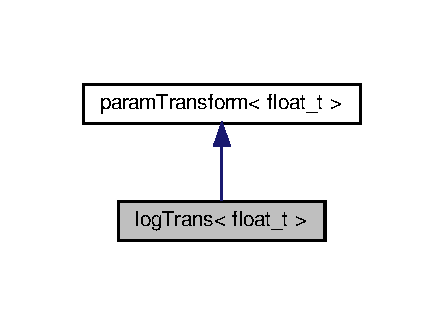
\includegraphics[width=168pt]{classlogTrans__inherit__graph}
\end{center}
\end{figure}


Collaboration diagram for log\+Trans\+:
\nopagebreak
\begin{figure}[H]
\begin{center}
\leavevmode
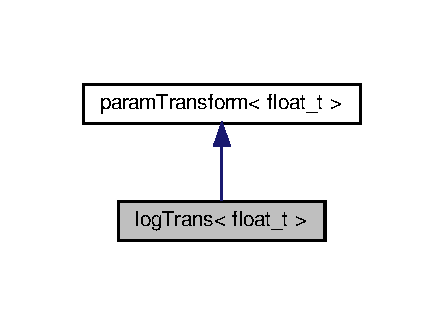
\includegraphics[width=168pt]{classlogTrans__coll__graph}
\end{center}
\end{figure}
\subsection*{Public Member Functions}
\begin{DoxyCompactItemize}
\item 
\mbox{\Hypertarget{classlogTrans_a091f99fe9fc1c85b73c5e1c220c6d227}\label{classlogTrans_a091f99fe9fc1c85b73c5e1c220c6d227}} 
double \hyperlink{classlogTrans_a091f99fe9fc1c85b73c5e1c220c6d227}{trans} (const double \&p) override
\begin{DoxyCompactList}\small\item\em from the constrained/nontransformed to the transformed/unconstrained space \end{DoxyCompactList}\item 
\mbox{\Hypertarget{classlogTrans_ae831a7d20e94dd80b8805a90b850e94a}\label{classlogTrans_ae831a7d20e94dd80b8805a90b850e94a}} 
double \hyperlink{classlogTrans_ae831a7d20e94dd80b8805a90b850e94a}{inv\+Trans} (const double \&trans\+\_\+p) override
\begin{DoxyCompactList}\small\item\em from the unconstrained/transformed to the constrained/untransformed space; \end{DoxyCompactList}\item 
\mbox{\Hypertarget{classlogTrans_af234991224cf994204ce196a85622ca8}\label{classlogTrans_af234991224cf994204ce196a85622ca8}} 
double \hyperlink{classlogTrans_af234991224cf994204ce196a85622ca8}{log\+Jacobian} (const double \&p) override
\begin{DoxyCompactList}\small\item\em get the log jacobian (from untransformed to transformed). For use with adjusting priors to the transformed space. \end{DoxyCompactList}\end{DoxyCompactItemize}
\subsection*{Additional Inherited Members}


The documentation for this class was generated from the following file\+:\begin{DoxyCompactItemize}
\item 
include/param\+\_\+transforms.\+h\end{DoxyCompactItemize}

\hypertarget{classnullTrans}{}\section{null\+Trans$<$ float\+\_\+t $>$ Class Template Reference}
\label{classnullTrans}\index{null\+Trans$<$ float\+\_\+t $>$@{null\+Trans$<$ float\+\_\+t $>$}}


{\ttfamily \#include $<$param\+\_\+transforms.\+h$>$}



Inheritance diagram for null\+Trans$<$ float\+\_\+t $>$\+:\nopagebreak
\begin{figure}[H]
\begin{center}
\leavevmode
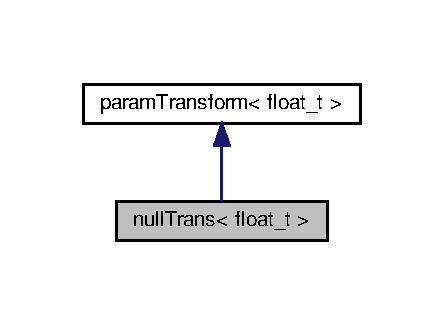
\includegraphics[width=213pt]{classnullTrans__inherit__graph}
\end{center}
\end{figure}


Collaboration diagram for null\+Trans$<$ float\+\_\+t $>$\+:\nopagebreak
\begin{figure}[H]
\begin{center}
\leavevmode
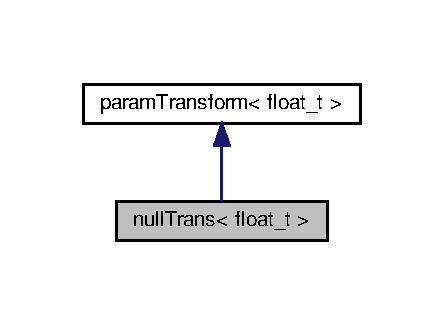
\includegraphics[width=213pt]{classnullTrans__coll__graph}
\end{center}
\end{figure}
\subsection*{Public Member Functions}
\begin{DoxyCompactItemize}
\item 
\mbox{\Hypertarget{classnullTrans_a908d4173fc1a56498fef91bd212b5b1f}\label{classnullTrans_a908d4173fc1a56498fef91bd212b5b1f}} 
float\+\_\+t \hyperlink{classnullTrans_a908d4173fc1a56498fef91bd212b5b1f}{trans} (const float\+\_\+t \&p) override
\begin{DoxyCompactList}\small\item\em from the constrained/nontransformed to the transformed/unconstrained space \end{DoxyCompactList}\item 
\mbox{\Hypertarget{classnullTrans_ac603661febf8ff99ccd79c682e050b1e}\label{classnullTrans_ac603661febf8ff99ccd79c682e050b1e}} 
float\+\_\+t \hyperlink{classnullTrans_ac603661febf8ff99ccd79c682e050b1e}{inv\+Trans} (const float\+\_\+t \&trans\+\_\+p) override
\begin{DoxyCompactList}\small\item\em from the unconstrained/transformed to the constrained/untransformed space; \end{DoxyCompactList}\item 
\mbox{\Hypertarget{classnullTrans_a12221c70fb73243de9133484b62406e8}\label{classnullTrans_a12221c70fb73243de9133484b62406e8}} 
float\+\_\+t \hyperlink{classnullTrans_a12221c70fb73243de9133484b62406e8}{log\+Jacobian} (const float\+\_\+t \&p) override
\begin{DoxyCompactList}\small\item\em get the log jacobian (from untransformed to transformed). For use with adjusting priors to the transformed space. \end{DoxyCompactList}\end{DoxyCompactItemize}
\subsection*{Additional Inherited Members}


\subsection{Detailed Description}
\subsubsection*{template$<$typename float\+\_\+t$>$\newline
class null\+Trans$<$ float\+\_\+t $>$}

\begin{DoxyAuthor}{Author}
t 
\end{DoxyAuthor}


The documentation for this class was generated from the following file\+:\begin{DoxyCompactItemize}
\item 
include/\hyperlink{param__transforms_8h}{param\+\_\+transforms.\+h}\end{DoxyCompactItemize}

\hypertarget{classparamPack}{}\section{param\+Pack Class Reference}
\label{classparamPack}\index{param\+Pack@{param\+Pack}}


{\ttfamily \#include $<$param\+\_\+pack.\+h$>$}

\subsection*{Public Types}
\begin{DoxyCompactItemize}
\item 
\mbox{\Hypertarget{classparamPack_a669db12cf2e7908255bf95bc1c46aafe}\label{classparamPack_a669db12cf2e7908255bf95bc1c46aafe}} 
using {\bfseries vecptrs} = std\+::vector$<$ std\+::unique\+\_\+ptr$<$ \hyperlink{classparamTransform}{param\+Transform} $>$ $>$
\end{DoxyCompactItemize}
\subsection*{Public Member Functions}
\begin{DoxyCompactItemize}
\item 
\mbox{\Hypertarget{classparamPack_a404c1db9bb4ebc258ac79200e1b92cf9}\label{classparamPack_a404c1db9bb4ebc258ac79200e1b92cf9}} 
{\bfseries param\+Pack} (const \hyperlink{classparamPack}{param\+Pack} \&pp)=delete
\item 
\mbox{\Hypertarget{classparamPack_a132baf34915216cae985ddcbff40cf75}\label{classparamPack_a132baf34915216cae985ddcbff40cf75}} 
{\bfseries param\+Pack} (const Eigen\+::\+Vector\+Xd \&trans\+\_\+params, vecptrs \&\&t\+\_\+functors)
\item 
\mbox{\Hypertarget{classparamPack_adc1cb981efe75da7e64fa279cd9ec467}\label{classparamPack_adc1cb981efe75da7e64fa279cd9ec467}} 
{\bfseries param\+Pack} (const Eigen\+::\+Vector\+Xd \&params, const std\+::vector$<$ Trans\+Type $>$ \&vec\+\_\+trans\+\_\+types, bool start\+\_\+w\+\_\+trans\+\_\+params=true)
\item 
\mbox{\Hypertarget{classparamPack_a14b86328a0a82a7d00b631fd79884e94}\label{classparamPack_a14b86328a0a82a7d00b631fd79884e94}} 
\hyperlink{classparamPack}{param\+Pack} \& {\bfseries operator=} (const \hyperlink{classparamPack}{param\+Pack} \&other)=delete
\item 
\mbox{\Hypertarget{classparamPack_a7374a7e3ea39a54d020fc91a3d971ffd}\label{classparamPack_a7374a7e3ea39a54d020fc91a3d971ffd}} 
\hyperlink{classparamPack}{param\+Pack} \& {\bfseries operator=} (\hyperlink{classparamPack}{param\+Pack} \&\&other)=delete
\item 
unsigned int \hyperlink{classparamPack_a69fc36c50f73e6b827d2e339e2e8b806}{get\+Num\+Params} () const
\begin{DoxyCompactList}\small\item\em get number of parameters \end{DoxyCompactList}\item 
Eigen\+::\+Vector\+Xd \hyperlink{classparamPack_a384545f4e43c572c236b2535514830e3}{get\+Trans\+Params} () const
\begin{DoxyCompactList}\small\item\em get the transformed parameters in the unrestricted space \end{DoxyCompactList}\item 
Eigen\+::\+Vector\+Xd \hyperlink{classparamPack_afd45bfe2c0c9d157df3f146d57bc492d}{get\+Un\+Trans\+Params} () const
\begin{DoxyCompactList}\small\item\em get the untransformed parameters in the possibly-\/restricted space \end{DoxyCompactList}\item 
Eigen\+::\+Vector\+Xd \hyperlink{classparamPack_aab8d550dbd4f28fce067197ba96f80fa}{get\+Trans\+Params} (const unsigned int \&start, const unsigned int \&end) const
\begin{DoxyCompactList}\small\item\em get a subset of the transformed parameters in the unrestricted space \end{DoxyCompactList}\item 
Eigen\+::\+Vector\+Xd \hyperlink{classparamPack_a0a2a21e73e3c8371e91db1b056317c46}{get\+Un\+Trans\+Params} (const unsigned int \&start, const unsigned int \&end) const
\begin{DoxyCompactList}\small\item\em get a subset of the untransformed parameters in the possibly-\/restricted space \end{DoxyCompactList}\item 
double \hyperlink{classparamPack_adb44adbc09eb281022984461fc2050f2}{get\+Log\+Jacobian} () const
\begin{DoxyCompactList}\small\item\em get the log of the Jacobian determinant you need for the density of transformed parameters. \end{DoxyCompactList}\item 
void \hyperlink{classparamPack_ac179e7541c993e05e5e435d5f20c558a}{take\+Values} (const \hyperlink{classparamPack}{param\+Pack} \&other)
\begin{DoxyCompactList}\small\item\em copy values from another \hyperlink{classparamPack}{param\+Pack} \end{DoxyCompactList}\end{DoxyCompactItemize}
\subsection*{Private Attributes}
\begin{DoxyCompactItemize}
\item 
\mbox{\Hypertarget{classparamPack_a3b341549b133b3f0ac47d6c600b7bcff}\label{classparamPack_a3b341549b133b3f0ac47d6c600b7bcff}} 
Eigen\+::\+Vector\+Xd {\bfseries m\+\_\+trans\+\_\+params}
\item 
\mbox{\Hypertarget{classparamPack_a8f9043bb2a179abb7ea707e36de2cfc1}\label{classparamPack_a8f9043bb2a179abb7ea707e36de2cfc1}} 
vecptrs {\bfseries m\+\_\+transform\+\_\+functors}
\end{DoxyCompactItemize}


\subsection{Detailed Description}
\begin{DoxyAuthor}{Author}
t 
\end{DoxyAuthor}


\subsection{Member Function Documentation}
\mbox{\Hypertarget{classparamPack_adb44adbc09eb281022984461fc2050f2}\label{classparamPack_adb44adbc09eb281022984461fc2050f2}} 
\index{param\+Pack@{param\+Pack}!get\+Log\+Jacobian@{get\+Log\+Jacobian}}
\index{get\+Log\+Jacobian@{get\+Log\+Jacobian}!param\+Pack@{param\+Pack}}
\subsubsection{\texorpdfstring{get\+Log\+Jacobian()}{getLogJacobian()}}
{\footnotesize\ttfamily double param\+Pack\+::get\+Log\+Jacobian (\begin{DoxyParamCaption}{ }\end{DoxyParamCaption}) const}



get the log of the Jacobian determinant you need for the density of transformed parameters. 

get the log of the Jacobian determinant you need for the density of transformed params \begin{DoxyReturn}{Returns}
a double 
\end{DoxyReturn}
\mbox{\Hypertarget{classparamPack_a69fc36c50f73e6b827d2e339e2e8b806}\label{classparamPack_a69fc36c50f73e6b827d2e339e2e8b806}} 
\index{param\+Pack@{param\+Pack}!get\+Num\+Params@{get\+Num\+Params}}
\index{get\+Num\+Params@{get\+Num\+Params}!param\+Pack@{param\+Pack}}
\subsubsection{\texorpdfstring{get\+Num\+Params()}{getNumParams()}}
{\footnotesize\ttfamily unsigned int param\+Pack\+::get\+Num\+Params (\begin{DoxyParamCaption}{ }\end{DoxyParamCaption}) const}



get number of parameters 

gets the number of parameters in your pack \begin{DoxyReturn}{Returns}
an unsigned integer 
\end{DoxyReturn}
\mbox{\Hypertarget{classparamPack_a384545f4e43c572c236b2535514830e3}\label{classparamPack_a384545f4e43c572c236b2535514830e3}} 
\index{param\+Pack@{param\+Pack}!get\+Trans\+Params@{get\+Trans\+Params}}
\index{get\+Trans\+Params@{get\+Trans\+Params}!param\+Pack@{param\+Pack}}
\subsubsection{\texorpdfstring{get\+Trans\+Params()}{getTransParams()}\hspace{0.1cm}{\footnotesize\ttfamily [1/2]}}
{\footnotesize\ttfamily Eigen\+::\+Vector\+Xd param\+Pack\+::get\+Trans\+Params (\begin{DoxyParamCaption}{ }\end{DoxyParamCaption}) const}



get the transformed parameters in the unrestricted space 

get the transformed parameters on the unrestricted space \begin{DoxyReturn}{Returns}
an Eigen\+::\+Vector of transformed parameters 
\end{DoxyReturn}
\mbox{\Hypertarget{classparamPack_aab8d550dbd4f28fce067197ba96f80fa}\label{classparamPack_aab8d550dbd4f28fce067197ba96f80fa}} 
\index{param\+Pack@{param\+Pack}!get\+Trans\+Params@{get\+Trans\+Params}}
\index{get\+Trans\+Params@{get\+Trans\+Params}!param\+Pack@{param\+Pack}}
\subsubsection{\texorpdfstring{get\+Trans\+Params()}{getTransParams()}\hspace{0.1cm}{\footnotesize\ttfamily [2/2]}}
{\footnotesize\ttfamily Eigen\+::\+Vector\+Xd param\+Pack\+::get\+Trans\+Params (\begin{DoxyParamCaption}\item[{const unsigned int \&}]{start,  }\item[{const unsigned int \&}]{end }\end{DoxyParamCaption}) const}



get a subset of the transformed parameters in the unrestricted space 

get a subset of the transformed parameters on the unrestricted space 
\begin{DoxyParams}{Parameters}
{\em index} & of first element (starts counting at zero) \\
\hline
{\em index} & of last element (not like python indexing!) \\
\hline
\end{DoxyParams}
\begin{DoxyReturn}{Returns}
an Eigen\+::\+Vector of transformed parameters 
\end{DoxyReturn}
\mbox{\Hypertarget{classparamPack_afd45bfe2c0c9d157df3f146d57bc492d}\label{classparamPack_afd45bfe2c0c9d157df3f146d57bc492d}} 
\index{param\+Pack@{param\+Pack}!get\+Un\+Trans\+Params@{get\+Un\+Trans\+Params}}
\index{get\+Un\+Trans\+Params@{get\+Un\+Trans\+Params}!param\+Pack@{param\+Pack}}
\subsubsection{\texorpdfstring{get\+Un\+Trans\+Params()}{getUnTransParams()}\hspace{0.1cm}{\footnotesize\ttfamily [1/2]}}
{\footnotesize\ttfamily Eigen\+::\+Vector\+Xd param\+Pack\+::get\+Un\+Trans\+Params (\begin{DoxyParamCaption}{ }\end{DoxyParamCaption}) const}



get the untransformed parameters in the possibly-\/restricted space 

get the untransformed parameters on the possibly-\/restricted space \begin{DoxyReturn}{Returns}
an Eigen\+::\+Vector of transformed parameters 
\end{DoxyReturn}
\mbox{\Hypertarget{classparamPack_a0a2a21e73e3c8371e91db1b056317c46}\label{classparamPack_a0a2a21e73e3c8371e91db1b056317c46}} 
\index{param\+Pack@{param\+Pack}!get\+Un\+Trans\+Params@{get\+Un\+Trans\+Params}}
\index{get\+Un\+Trans\+Params@{get\+Un\+Trans\+Params}!param\+Pack@{param\+Pack}}
\subsubsection{\texorpdfstring{get\+Un\+Trans\+Params()}{getUnTransParams()}\hspace{0.1cm}{\footnotesize\ttfamily [2/2]}}
{\footnotesize\ttfamily Eigen\+::\+Vector\+Xd param\+Pack\+::get\+Un\+Trans\+Params (\begin{DoxyParamCaption}\item[{const unsigned int \&}]{start,  }\item[{const unsigned int \&}]{end }\end{DoxyParamCaption}) const}



get a subset of the untransformed parameters in the possibly-\/restricted space 

get a subset of the transformed parameters on the unrestricted space 
\begin{DoxyParams}{Parameters}
{\em index} & of first element (starts counting at zero) \\
\hline
{\em index} & of last element (not like python indexing!) \\
\hline
\end{DoxyParams}
\begin{DoxyReturn}{Returns}
an Eigen\+::\+Vector of transformed parameters 
\end{DoxyReturn}
\mbox{\Hypertarget{classparamPack_ac179e7541c993e05e5e435d5f20c558a}\label{classparamPack_ac179e7541c993e05e5e435d5f20c558a}} 
\index{param\+Pack@{param\+Pack}!take\+Values@{take\+Values}}
\index{take\+Values@{take\+Values}!param\+Pack@{param\+Pack}}
\subsubsection{\texorpdfstring{take\+Values()}{takeValues()}}
{\footnotesize\ttfamily void param\+Pack\+::take\+Values (\begin{DoxyParamCaption}\item[{const \hyperlink{classparamPack}{param\+Pack} \&}]{other }\end{DoxyParamCaption})}



copy values from another \hyperlink{classparamPack}{param\+Pack} 

copy the values of another \hyperlink{classparamPack}{param\+Pack} 
\begin{DoxyParams}{Parameters}
{\em the} & other parameter pack whose values you want to take as your own \\
\hline
\end{DoxyParams}


The documentation for this class was generated from the following file\+:\begin{DoxyCompactItemize}
\item 
include/\hyperlink{param__pack_8h}{param\+\_\+pack.\+h}\end{DoxyCompactItemize}

\hypertarget{classparamTransform}{}\section{param\+Transform Class Reference}
\label{classparamTransform}\index{param\+Transform@{param\+Transform}}


Inheritance diagram for param\+Transform\+:
\nopagebreak
\begin{figure}[H]
\begin{center}
\leavevmode
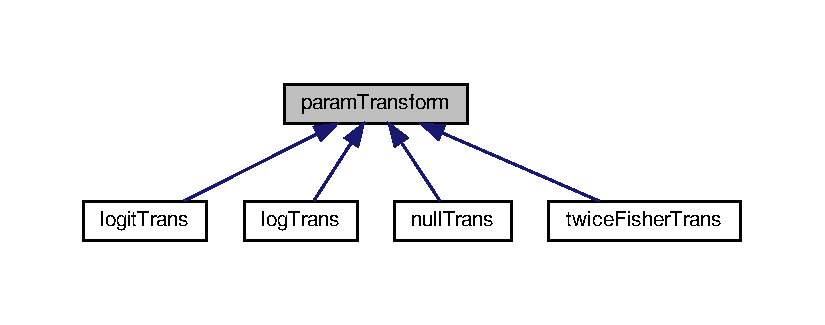
\includegraphics[width=350pt]{classparamTransform__inherit__graph}
\end{center}
\end{figure}
\subsection*{Public Member Functions}
\begin{DoxyCompactItemize}
\item 
\mbox{\Hypertarget{classparamTransform_a7eaa549e2a14fe05080378a5967d9c97}\label{classparamTransform_a7eaa549e2a14fe05080378a5967d9c97}} 
virtual \hyperlink{classparamTransform_a7eaa549e2a14fe05080378a5967d9c97}{$\sim$param\+Transform} ()
\begin{DoxyCompactList}\small\item\em a virtual destructor \end{DoxyCompactList}\item 
\mbox{\Hypertarget{classparamTransform_a0f380ca288488f76f15819704920bf27}\label{classparamTransform_a0f380ca288488f76f15819704920bf27}} 
virtual double \hyperlink{classparamTransform_a0f380ca288488f76f15819704920bf27}{trans} (const double \&p)=0
\begin{DoxyCompactList}\small\item\em from the constrained/nontransformed to the transformed/unconstrained space \end{DoxyCompactList}\item 
\mbox{\Hypertarget{classparamTransform_a183baf22182cddc645567ee202a895fc}\label{classparamTransform_a183baf22182cddc645567ee202a895fc}} 
virtual double \hyperlink{classparamTransform_a183baf22182cddc645567ee202a895fc}{inv\+Trans} (const double \&trans\+\_\+p)=0
\begin{DoxyCompactList}\small\item\em from the unconstrained/transformed to the constrained/untransformed space; \end{DoxyCompactList}\item 
\mbox{\Hypertarget{classparamTransform_a0b30b6b43073c589a1f48a61b2c0d77f}\label{classparamTransform_a0b30b6b43073c589a1f48a61b2c0d77f}} 
virtual double \hyperlink{classparamTransform_a0b30b6b43073c589a1f48a61b2c0d77f}{log\+Jacobian} (const double \&p)=0
\begin{DoxyCompactList}\small\item\em get the log jacobian (from untransformed to transformed). For use with adjusting priors to the transformed space. \end{DoxyCompactList}\end{DoxyCompactItemize}
\subsection*{Static Public Member Functions}
\begin{DoxyCompactItemize}
\item 
\mbox{\Hypertarget{classparamTransform_a3cef2dd407ed30c66ff9a5cab8516a3c}\label{classparamTransform_a3cef2dd407ed30c66ff9a5cab8516a3c}} 
static std\+::unique\+\_\+ptr$<$ \hyperlink{classparamTransform}{param\+Transform} $>$ \hyperlink{classparamTransform_a3cef2dd407ed30c66ff9a5cab8516a3c}{create} (Trans\+Type tt)
\begin{DoxyCompactList}\small\item\em a static method to create unique pointers \end{DoxyCompactList}\end{DoxyCompactItemize}


The documentation for this class was generated from the following file\+:\begin{DoxyCompactItemize}
\item 
include/param\+\_\+transforms.\+h\end{DoxyCompactItemize}

\hypertarget{classsvol__bs}{}\doxysection{svol\+\_\+bs$<$ nparts, dimx, dimy, resampT, float\+\_\+t $>$ Class Template Reference}
\label{classsvol__bs}\index{svol\_bs$<$ nparts, dimx, dimy, resampT, float\_t $>$@{svol\_bs$<$ nparts, dimx, dimy, resampT, float\_t $>$}}


Inheritance diagram for svol\+\_\+bs$<$ nparts, dimx, dimy, resampT, float\+\_\+t $>$\+:
\nopagebreak
\begin{figure}[H]
\begin{center}
\leavevmode
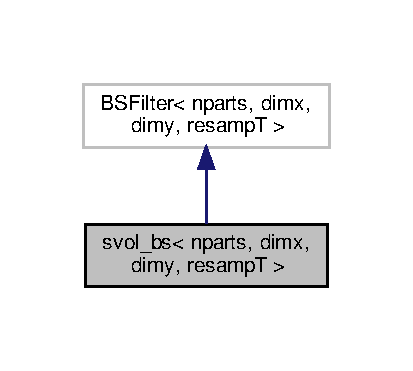
\includegraphics[width=221pt]{classsvol__bs__inherit__graph}
\end{center}
\end{figure}


Collaboration diagram for svol\+\_\+bs$<$ nparts, dimx, dimy, resampT, float\+\_\+t $>$\+:
\nopagebreak
\begin{figure}[H]
\begin{center}
\leavevmode
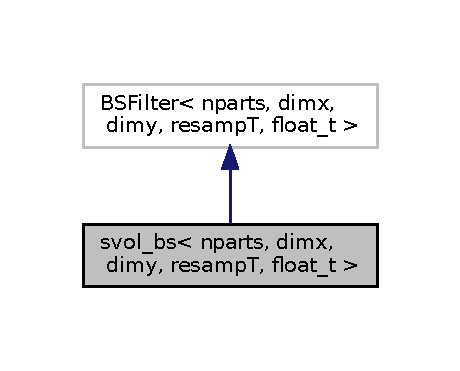
\includegraphics[width=221pt]{classsvol__bs__coll__graph}
\end{center}
\end{figure}
\doxysubsection*{Public Types}
\begin{DoxyCompactItemize}
\item 
\mbox{\Hypertarget{classsvol__bs_a8ef6370aa347e276147b393786a7ecd5}\label{classsvol__bs_a8ef6370aa347e276147b393786a7ecd5}} 
using {\bfseries ssv} = Eigen\+::\+Matrix$<$ float\+\_\+t, dimx, 1 $>$
\item 
\mbox{\Hypertarget{classsvol__bs_a90e38a1fae511361b0ac017b0c5c80a0}\label{classsvol__bs_a90e38a1fae511361b0ac017b0c5c80a0}} 
using {\bfseries osv} = Eigen\+::\+Matrix$<$ float\+\_\+t, dimy, 1 $>$
\end{DoxyCompactItemize}
\doxysubsection*{Public Member Functions}
\begin{DoxyCompactItemize}
\item 
\mbox{\Hypertarget{classsvol__bs_a36902082260b8fb13251722ac8b527a8}\label{classsvol__bs_a36902082260b8fb13251722ac8b527a8}} 
{\bfseries svol\+\_\+bs} (const float\+\_\+t \&phi, const float\+\_\+t \&beta, const float\+\_\+t \&sigma)
\item 
\mbox{\Hypertarget{classsvol__bs_a805744b065f42b9099a29890f8f029dc}\label{classsvol__bs_a805744b065f42b9099a29890f8f029dc}} 
{\bfseries svol\+\_\+bs} (const \mbox{\hyperlink{classparam_1_1pack}{param\+::pack}}$<$ float\+\_\+t, 3 $>$ \&pp)
\item 
\mbox{\Hypertarget{classsvol__bs_a4461faab02ba3fa09ee9e4977841b297}\label{classsvol__bs_a4461faab02ba3fa09ee9e4977841b297}} 
float\+\_\+t {\bfseries log\+Q1\+Ev} (const ssv \&x1, const osv \&y1)
\item 
\mbox{\Hypertarget{classsvol__bs_a067870660bf0d60b032411df7fe32546}\label{classsvol__bs_a067870660bf0d60b032411df7fe32546}} 
float\+\_\+t {\bfseries log\+Mu\+Ev} (const ssv \&x1)
\item 
\mbox{\Hypertarget{classsvol__bs_a460a24a129edaf68650aeec9d28fedf8}\label{classsvol__bs_a460a24a129edaf68650aeec9d28fedf8}} 
float\+\_\+t {\bfseries log\+G\+Ev} (const osv \&yt, const ssv \&xt)
\item 
\mbox{\Hypertarget{classsvol__bs_a59120c1870072f1d63a3057d9ba614cf}\label{classsvol__bs_a59120c1870072f1d63a3057d9ba614cf}} 
auto {\bfseries f\+Samp} (const ssv \&xtm1) -\/$>$ ssv
\item 
\mbox{\Hypertarget{classsvol__bs_ab12997187805f7d9b21f5041daaf70b7}\label{classsvol__bs_ab12997187805f7d9b21f5041daaf70b7}} 
auto {\bfseries q1\+Samp} (const osv \&y1) -\/$>$ ssv
\end{DoxyCompactItemize}
\doxysubsection*{Public Attributes}
\begin{DoxyCompactItemize}
\item 
\mbox{\Hypertarget{classsvol__bs_ab46db50cdce58fd3b9d72566dfc12715}\label{classsvol__bs_ab46db50cdce58fd3b9d72566dfc12715}} 
float\+\_\+t {\bfseries m\+\_\+phi}
\item 
\mbox{\Hypertarget{classsvol__bs_ae197d739aedd1c2df113f2de6131495c}\label{classsvol__bs_ae197d739aedd1c2df113f2de6131495c}} 
float\+\_\+t {\bfseries m\+\_\+beta}
\item 
\mbox{\Hypertarget{classsvol__bs_aa312d7aa75de3c1d42c023a2ff8d63b5}\label{classsvol__bs_aa312d7aa75de3c1d42c023a2ff8d63b5}} 
float\+\_\+t {\bfseries m\+\_\+sigma}
\item 
\mbox{\Hypertarget{classsvol__bs_a324a11de663832348bf3ce3435a1b0df}\label{classsvol__bs_a324a11de663832348bf3ce3435a1b0df}} 
rvsamp\+::\+Univ\+Norm\+Sampler$<$ float\+\_\+t $>$ {\bfseries m\+\_\+std\+Norm\+Sampler}
\end{DoxyCompactItemize}


The documentation for this class was generated from the following file\+:\begin{DoxyCompactItemize}
\item 
example/univ\+\_\+svol\+\_\+bootstrap\+\_\+filter.\+h\end{DoxyCompactItemize}

\hypertarget{classtwiceFisherTrans}{}\section{twice\+Fisher\+Trans Class Reference}
\label{classtwiceFisherTrans}\index{twice\+Fisher\+Trans@{twice\+Fisher\+Trans}}


Inheritance diagram for twice\+Fisher\+Trans\+:
\nopagebreak
\begin{figure}[H]
\begin{center}
\leavevmode
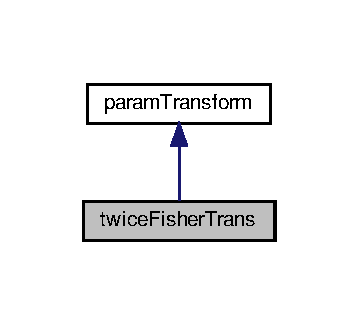
\includegraphics[width=172pt]{classtwiceFisherTrans__inherit__graph}
\end{center}
\end{figure}


Collaboration diagram for twice\+Fisher\+Trans\+:
\nopagebreak
\begin{figure}[H]
\begin{center}
\leavevmode
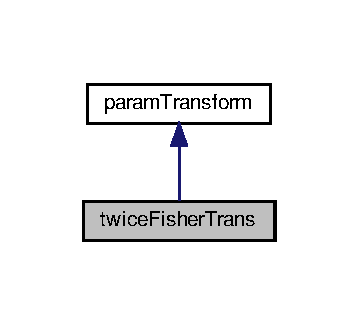
\includegraphics[width=172pt]{classtwiceFisherTrans__coll__graph}
\end{center}
\end{figure}
\subsection*{Public Member Functions}
\begin{DoxyCompactItemize}
\item 
\mbox{\Hypertarget{classtwiceFisherTrans_aaf4a8e1af5f96d546ddfb820668991af}\label{classtwiceFisherTrans_aaf4a8e1af5f96d546ddfb820668991af}} 
double \hyperlink{classtwiceFisherTrans_aaf4a8e1af5f96d546ddfb820668991af}{trans} (const double \&p) override
\begin{DoxyCompactList}\small\item\em from the constrained/nontransformed to the transformed/unconstrained space \end{DoxyCompactList}\item 
\mbox{\Hypertarget{classtwiceFisherTrans_a5bdcbf4f98e6ac10f4b28aa067db3f0d}\label{classtwiceFisherTrans_a5bdcbf4f98e6ac10f4b28aa067db3f0d}} 
double \hyperlink{classtwiceFisherTrans_a5bdcbf4f98e6ac10f4b28aa067db3f0d}{inv\+Trans} (const double \&trans\+\_\+p) override
\begin{DoxyCompactList}\small\item\em from the unconstrained/transformed to the constrained/untransformed space; \end{DoxyCompactList}\item 
\mbox{\Hypertarget{classtwiceFisherTrans_a134740afe211efd97f0cb078e51d278d}\label{classtwiceFisherTrans_a134740afe211efd97f0cb078e51d278d}} 
double \hyperlink{classtwiceFisherTrans_a134740afe211efd97f0cb078e51d278d}{log\+Jacobian} (const double \&p) override
\begin{DoxyCompactList}\small\item\em get the log jacobian (from untransformed to transformed). For use with adjusting priors to the transformed space. \end{DoxyCompactList}\end{DoxyCompactItemize}
\subsection*{Additional Inherited Members}


The documentation for this class was generated from the following file\+:\begin{DoxyCompactItemize}
\item 
include/param\+\_\+transforms.\+h\end{DoxyCompactItemize}

\hypertarget{classuniv__svol__estimator}{}\section{univ\+\_\+svol\+\_\+estimator$<$ numparams, dimstate, dimobs, numparts, float\+\_\+t $>$ Class Template Reference}
\label{classuniv__svol__estimator}\index{univ\+\_\+svol\+\_\+estimator$<$ numparams, dimstate, dimobs, numparts, float\+\_\+t $>$@{univ\+\_\+svol\+\_\+estimator$<$ numparams, dimstate, dimobs, numparts, float\+\_\+t $>$}}


Inheritance diagram for univ\+\_\+svol\+\_\+estimator$<$ numparams, dimstate, dimobs, numparts, float\+\_\+t $>$\+:\nopagebreak
\begin{figure}[H]
\begin{center}
\leavevmode
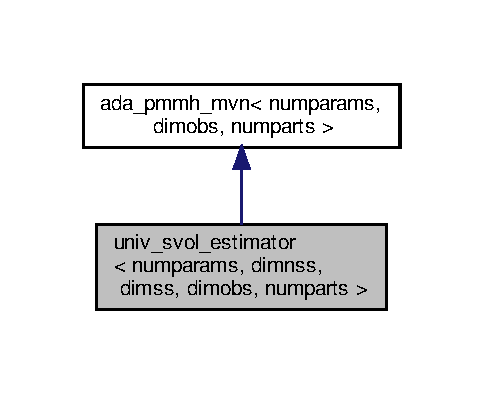
\includegraphics[width=232pt]{classuniv__svol__estimator__inherit__graph}
\end{center}
\end{figure}


Collaboration diagram for univ\+\_\+svol\+\_\+estimator$<$ numparams, dimstate, dimobs, numparts, float\+\_\+t $>$\+:\nopagebreak
\begin{figure}[H]
\begin{center}
\leavevmode
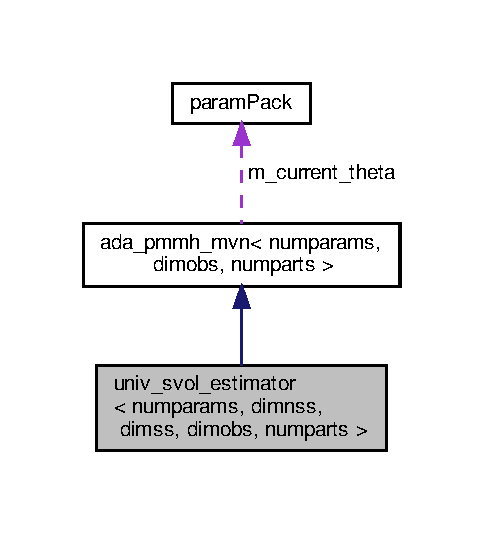
\includegraphics[width=232pt]{classuniv__svol__estimator__coll__graph}
\end{center}
\end{figure}
\subsection*{Public Types}
\begin{DoxyCompactItemize}
\item 
\mbox{\Hypertarget{classuniv__svol__estimator_a01b200275c33196fc939700e2ae2cae8}\label{classuniv__svol__estimator_a01b200275c33196fc939700e2ae2cae8}} 
using {\bfseries psv} = Eigen\+::\+Matrix$<$ float\+\_\+t, numparams, 1 $>$
\item 
\mbox{\Hypertarget{classuniv__svol__estimator_a49cb877a0ab3ac89cd59659ff4100e4c}\label{classuniv__svol__estimator_a49cb877a0ab3ac89cd59659ff4100e4c}} 
using {\bfseries psm} = Eigen\+::\+Matrix$<$ float\+\_\+t, numparams, numparams $>$
\item 
\mbox{\Hypertarget{classuniv__svol__estimator_ae88faafe9c8b75708d18260c0f4740a4}\label{classuniv__svol__estimator_ae88faafe9c8b75708d18260c0f4740a4}} 
using {\bfseries osv} = Eigen\+::\+Matrix$<$ float\+\_\+t, dimobs, 1 $>$
\end{DoxyCompactItemize}
\subsection*{Public Member Functions}
\begin{DoxyCompactItemize}
\item 
\mbox{\Hypertarget{classuniv__svol__estimator_a16694966fefdaef94dcee68e961cf978}\label{classuniv__svol__estimator_a16694966fefdaef94dcee68e961cf978}} 
{\bfseries univ\+\_\+svol\+\_\+estimator} (const psv \&start\+Trans\+Theta, const std\+::vector$<$ \hyperlink{param__transforms_8h_acee593b112f4fc85f850631b9c6aaae9}{Trans\+Type} $>$ \&tts, const unsigned int \&num\+M\+C\+M\+C\+Iters, const std\+::string \&data\+File, const std\+::string \&samples\+\_\+base\+\_\+name, const std\+::string \&messages\+\_\+base\+\_\+name, const bool \&mc, const unsigned int \&t0, const unsigned int \&t1, const psm \&C0, bool print\+\_\+to\+\_\+console, unsigned int print\+\_\+every\+\_\+k)
\item 
float\+\_\+t \hyperlink{classuniv__svol__estimator_a2e0e55bf061ca8f59fa5d42ae6495fdd}{log\+Prior\+Evaluate} (const \hyperlink{classparamPack}{param\+Pack}$<$ float\+\_\+t $>$ \&theta)
\begin{DoxyCompactList}\small\item\em Evaluates the log of the model\textquotesingle{}s prior distribution assuming the original/nontransformed/contrained parameterization. \end{DoxyCompactList}\item 
float\+\_\+t \hyperlink{classuniv__svol__estimator_a1223321e7875a4d40f9c4817753a2e01}{log\+Like\+Evaluate} (const \hyperlink{classparamPack}{param\+Pack}$<$ float\+\_\+t $>$ \&theta, const std\+::vector$<$ osv $>$ \&data)
\begin{DoxyCompactList}\small\item\em Evaluates (approximates) the log-\/likelihood with a particle filter. \end{DoxyCompactList}\end{DoxyCompactItemize}


\subsection{Member Function Documentation}
\mbox{\Hypertarget{classuniv__svol__estimator_a1223321e7875a4d40f9c4817753a2e01}\label{classuniv__svol__estimator_a1223321e7875a4d40f9c4817753a2e01}} 
\index{univ\+\_\+svol\+\_\+estimator@{univ\+\_\+svol\+\_\+estimator}!log\+Like\+Evaluate@{log\+Like\+Evaluate}}
\index{log\+Like\+Evaluate@{log\+Like\+Evaluate}!univ\+\_\+svol\+\_\+estimator@{univ\+\_\+svol\+\_\+estimator}}
\subsubsection{\texorpdfstring{log\+Like\+Evaluate()}{logLikeEvaluate()}}
{\footnotesize\ttfamily template$<$size\+\_\+t numparams, size\+\_\+t dimstate, size\+\_\+t dimobs, size\+\_\+t numparts, typename float\+\_\+t $>$ \\
float\+\_\+t \hyperlink{classuniv__svol__estimator}{univ\+\_\+svol\+\_\+estimator}$<$ numparams, dimstate, dimobs, numparts, float\+\_\+t $>$\+::log\+Like\+Evaluate (\begin{DoxyParamCaption}\item[{const \hyperlink{classparamPack}{param\+Pack}$<$ float\+\_\+t $>$ \&}]{theta,  }\item[{const std\+::vector$<$ osv $>$ \&}]{data }\end{DoxyParamCaption})\hspace{0.3cm}{\ttfamily [virtual]}}



Evaluates (approximates) the log-\/likelihood with a particle filter. 


\begin{DoxyParams}{Parameters}
{\em theta} & the parameters with which to run the particle filter. \\
\hline
{\em data} & the observed data with which to run the particle filter. \\
\hline
\end{DoxyParams}
\begin{DoxyReturn}{Returns}
the evaluation (as a float\+\_\+t) of the log likelihood approximation. 
\end{DoxyReturn}


Implements \hyperlink{classada__pmmh__mvn_a82d43085173fd0ed33ee42de9be48b77}{ada\+\_\+pmmh\+\_\+mvn$<$ numparams, dimobs, numparts, float\+\_\+t $>$}.

\mbox{\Hypertarget{classuniv__svol__estimator_a2e0e55bf061ca8f59fa5d42ae6495fdd}\label{classuniv__svol__estimator_a2e0e55bf061ca8f59fa5d42ae6495fdd}} 
\index{univ\+\_\+svol\+\_\+estimator@{univ\+\_\+svol\+\_\+estimator}!log\+Prior\+Evaluate@{log\+Prior\+Evaluate}}
\index{log\+Prior\+Evaluate@{log\+Prior\+Evaluate}!univ\+\_\+svol\+\_\+estimator@{univ\+\_\+svol\+\_\+estimator}}
\subsubsection{\texorpdfstring{log\+Prior\+Evaluate()}{logPriorEvaluate()}}
{\footnotesize\ttfamily template$<$size\+\_\+t numparams, size\+\_\+t dimstate, size\+\_\+t dimobs, size\+\_\+t numparts, typename float\+\_\+t $>$ \\
float\+\_\+t \hyperlink{classuniv__svol__estimator}{univ\+\_\+svol\+\_\+estimator}$<$ numparams, dimstate, dimobs, numparts, float\+\_\+t $>$\+::log\+Prior\+Evaluate (\begin{DoxyParamCaption}\item[{const \hyperlink{classparamPack}{param\+Pack}$<$ float\+\_\+t $>$ \&}]{theta }\end{DoxyParamCaption})\hspace{0.3cm}{\ttfamily [virtual]}}



Evaluates the log of the model\textquotesingle{}s prior distribution assuming the original/nontransformed/contrained parameterization. 


\begin{DoxyParams}{Parameters}
{\em theta} & the parameters argument (nontransformed/constrained parameterization). \\
\hline
\end{DoxyParams}
\begin{DoxyReturn}{Returns}
the log of the prior density. 
\end{DoxyReturn}


Implements \hyperlink{classada__pmmh__mvn_af946eae70a63045515ed7830c35106dc}{ada\+\_\+pmmh\+\_\+mvn$<$ numparams, dimobs, numparts, float\+\_\+t $>$}.



The documentation for this class was generated from the following file\+:\begin{DoxyCompactItemize}
\item 
example/estimate\+\_\+univ\+\_\+svol.\+h\end{DoxyCompactItemize}

\chapter{File Documentation}
\hypertarget{ada__pmmh_8h}{}\section{include/ada\+\_\+pmmh.h File Reference}
\label{ada__pmmh_8h}\index{include/ada\+\_\+pmmh.\+h@{include/ada\+\_\+pmmh.\+h}}


Performs an adaptive version of the particle marginal Metropilis-\/\+Hastings algorithm. The user is asked to design his/her own proposal density and prior distribution. The sampling is handled on an \char`\"{}as-\/is\char`\"{} basis, which means that it is entirely the user\textquotesingle{}s own responsibility to decide on what parameterization to use, to handle Jacobians if they are necessary, etc. These parameters will be written in an \char`\"{}as-\/is\char`\"{} fashion, as well. These calculations can be facilitates using the {\ttfamily \hyperlink{classparamPack}{param\+Pack}} class, however using this class is not absolutely necessary. Also, for convenience, a moving average covariance matrix estimate is performed; however, this should be ignored if the user is not interested in adaptive M\+C\+MC or isn\textquotesingle{}t using a transformed parameter space.  


{\ttfamily \#include $<$vector$>$}\newline
{\ttfamily \#include $<$Eigen/\+Dense$>$}\newline
{\ttfamily \#include $<$iostream$>$}\newline
{\ttfamily \#include $<$thread$>$}\newline
{\ttfamily \#include $<$atomic$>$}\newline
{\ttfamily \#include $<$fstream$>$}\newline
{\ttfamily \#include $<$future$>$}\newline
{\ttfamily \#include \char`\"{}rv\+\_\+samp.\+h\char`\"{}}\newline
{\ttfamily \#include \char`\"{}utils.\+h\char`\"{}}\newline
Include dependency graph for ada\+\_\+pmmh.\+h\+:\nopagebreak
\begin{figure}[H]
\begin{center}
\leavevmode
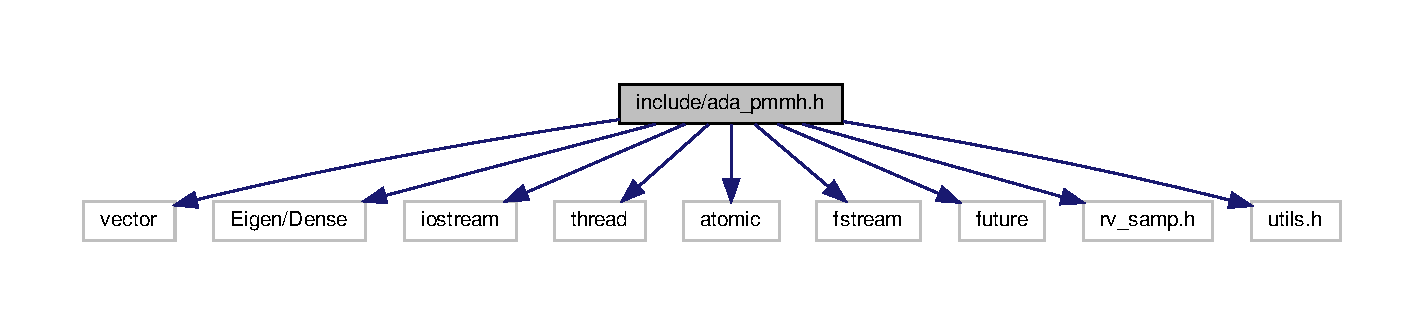
\includegraphics[width=350pt]{ada__pmmh_8h__incl}
\end{center}
\end{figure}
\subsection*{Classes}
\begin{DoxyCompactItemize}
\item 
class \hyperlink{classada__pmmh}{ada\+\_\+pmmh$<$ numparams, dimobs, numparts, float\+\_\+t $>$}
\end{DoxyCompactItemize}


\subsection{Detailed Description}
Performs an adaptive version of the particle marginal Metropilis-\/\+Hastings algorithm. The user is asked to design his/her own proposal density and prior distribution. The sampling is handled on an \char`\"{}as-\/is\char`\"{} basis, which means that it is entirely the user\textquotesingle{}s own responsibility to decide on what parameterization to use, to handle Jacobians if they are necessary, etc. These parameters will be written in an \char`\"{}as-\/is\char`\"{} fashion, as well. These calculations can be facilitates using the {\ttfamily \hyperlink{classparamPack}{param\+Pack}} class, however using this class is not absolutely necessary. Also, for convenience, a moving average covariance matrix estimate is performed; however, this should be ignored if the user is not interested in adaptive M\+C\+MC or isn\textquotesingle{}t using a transformed parameter space. 


\hypertarget{ada__pmmh__mvn_8h}{}\section{include/ada\+\_\+pmmh\+\_\+mvn.h File Reference}
\label{ada__pmmh__mvn_8h}\index{include/ada\+\_\+pmmh\+\_\+mvn.\+h@{include/ada\+\_\+pmmh\+\_\+mvn.\+h}}


Performs adaptive particle marginal metropolis-\/hastings sampling, using a multivariate normal distribution as the proposal. This samples on the transformed space, but it writes the the untransformed/constrained samples to the output. The priors requested by the user are for the (hopefully more convenient) un-\/transformed or constrainedspace. This means that the user never has to worry about handling any kind of Jacobian.  


{\ttfamily \#include $<$vector$>$}\newline
{\ttfamily \#include $<$Eigen/\+Dense$>$}\newline
{\ttfamily \#include $<$iostream$>$}\newline
{\ttfamily \#include $<$thread$>$}\newline
{\ttfamily \#include $<$atomic$>$}\newline
{\ttfamily \#include $<$fstream$>$}\newline
{\ttfamily \#include $<$future$>$}\newline
{\ttfamily \#include $<$chrono$>$}\newline
{\ttfamily \#include $<$typeinfo$>$}\newline
{\ttfamily \#include \char`\"{}rv\+\_\+eval.\+h\char`\"{}}\newline
{\ttfamily \#include \char`\"{}rv\+\_\+samp.\+h\char`\"{}}\newline
{\ttfamily \#include \char`\"{}utils.\+h\char`\"{}}\newline
{\ttfamily \#include \char`\"{}param\+\_\+pack.\+h\char`\"{}}\newline
Include dependency graph for ada\+\_\+pmmh\+\_\+mvn.\+h\+:
\nopagebreak
\begin{figure}[H]
\begin{center}
\leavevmode
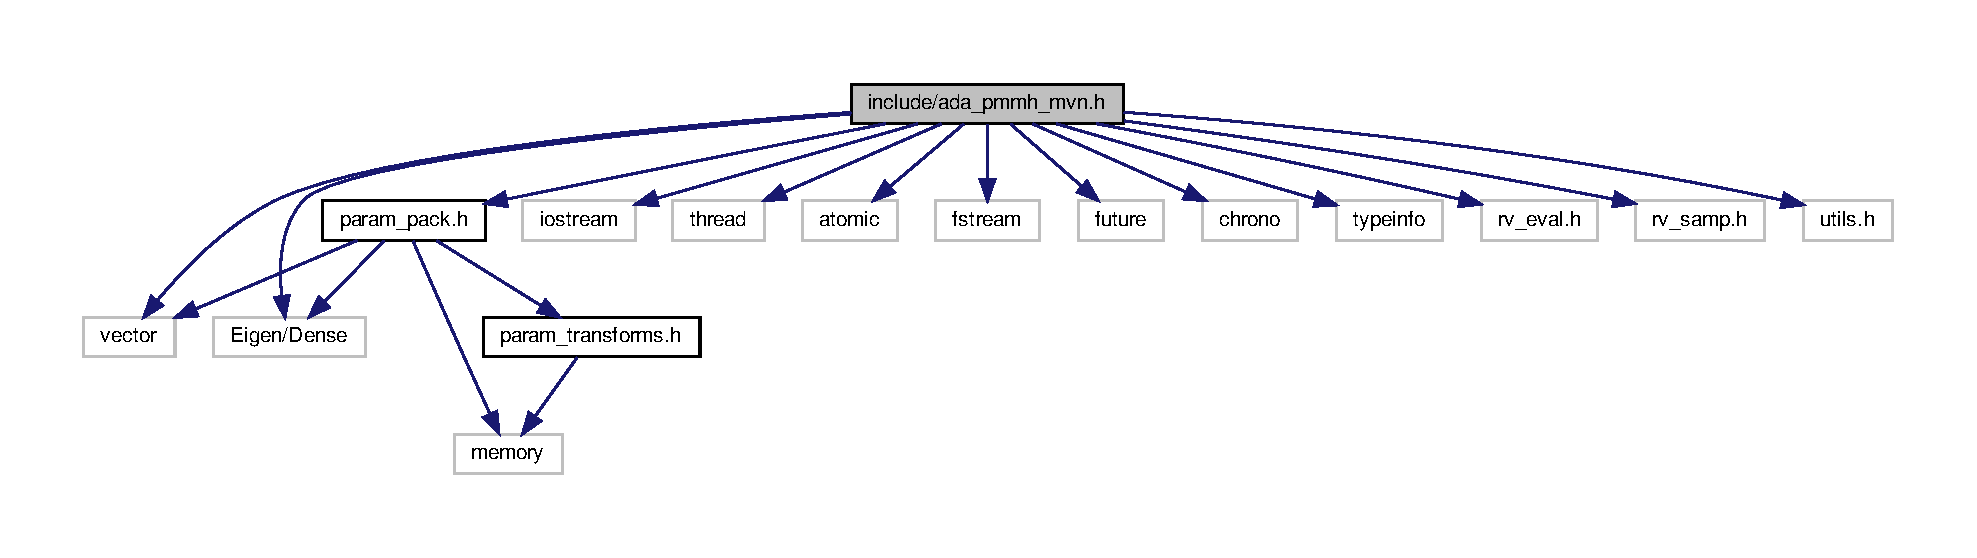
\includegraphics[width=350pt]{ada__pmmh__mvn_8h__incl}
\end{center}
\end{figure}
This graph shows which files directly or indirectly include this file\+:
\nopagebreak
\begin{figure}[H]
\begin{center}
\leavevmode
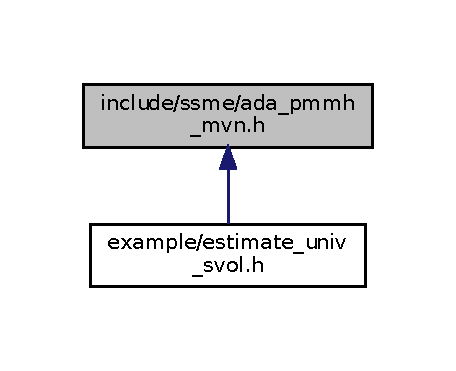
\includegraphics[width=211pt]{ada__pmmh__mvn_8h__dep__incl}
\end{center}
\end{figure}
\subsection*{Classes}
\begin{DoxyCompactItemize}
\item 
class \hyperlink{classada__pmmh__mvn}{ada\+\_\+pmmh\+\_\+mvn$<$ numparams, dimobs, numparts $>$}
\end{DoxyCompactItemize}


\subsection{Detailed Description}
Performs adaptive particle marginal metropolis-\/hastings sampling, using a multivariate normal distribution as the proposal. This samples on the transformed space, but it writes the the untransformed/constrained samples to the output. The priors requested by the user are for the (hopefully more convenient) un-\/transformed or constrainedspace. This means that the user never has to worry about handling any kind of Jacobian. 


\hypertarget{ada__rwmh_8h}{}\section{include/ada\+\_\+rwmh.h File Reference}
\label{ada__rwmh_8h}\index{include/ada\+\_\+rwmh.\+h@{include/ada\+\_\+rwmh.\+h}}


Performs adaptive random walk metropolis-\/hastings sampling (uses a multivariate normal distribution as the proposal). This samples on the transformed space, but it writes the untransformed/constrained samples to the output. The priors requested by the user are for the (more convenient) un-\/transformed aka constrained space. This means that the user never has to worry about handling any kind of Jacobian.  


{\ttfamily \#include $<$vector$>$}\newline
{\ttfamily \#include $<$Eigen/\+Dense$>$}\newline
{\ttfamily \#include $<$iostream$>$}\newline
{\ttfamily \#include $<$fstream$>$}\newline
{\ttfamily \#include $<$chrono$>$}\newline
{\ttfamily \#include \char`\"{}rv\+\_\+eval.\+h\char`\"{}}\newline
{\ttfamily \#include \char`\"{}rv\+\_\+samp.\+h\char`\"{}}\newline
{\ttfamily \#include \char`\"{}utils.\+h\char`\"{}}\newline
{\ttfamily \#include \char`\"{}param\+\_\+pack.\+h\char`\"{}}\newline
Include dependency graph for ada\+\_\+rwmh.\+h\+:
\nopagebreak
\begin{figure}[H]
\begin{center}
\leavevmode
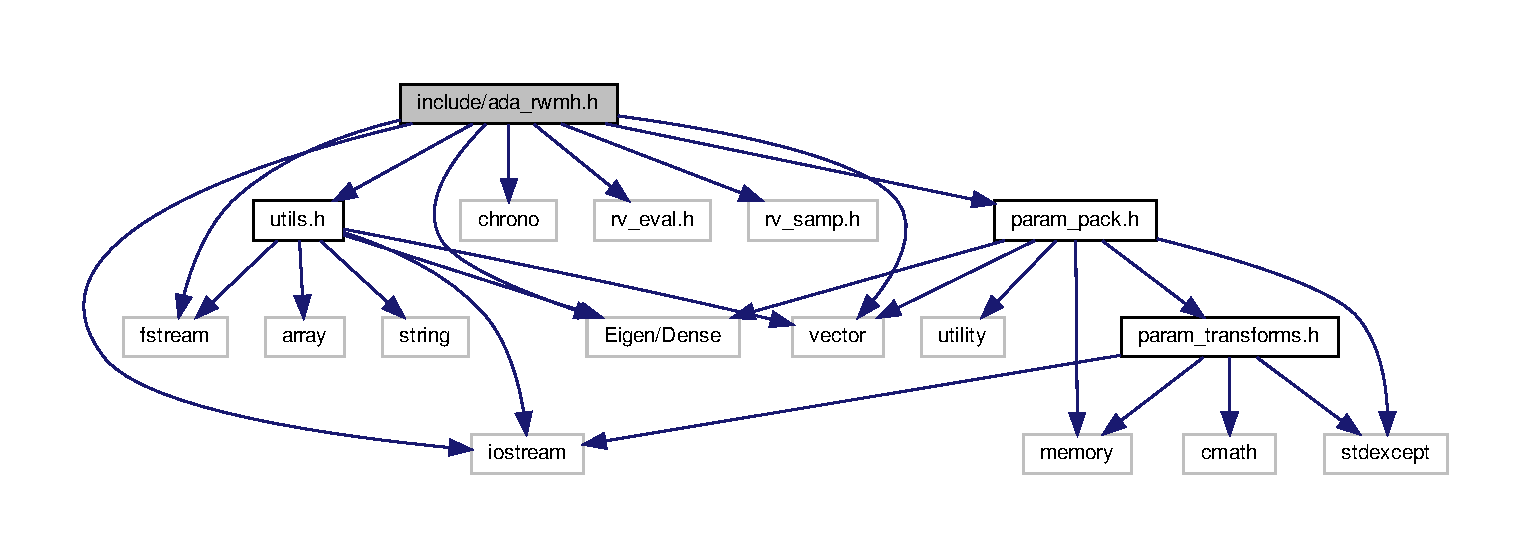
\includegraphics[width=350pt]{ada__rwmh_8h__incl}
\end{center}
\end{figure}
\subsection*{Classes}
\begin{DoxyCompactItemize}
\item 
class \hyperlink{classada__rwmh}{ada\+\_\+rwmh$<$ numparams, dimobs, float\+\_\+t $>$}
\end{DoxyCompactItemize}


\subsection{Detailed Description}
Performs adaptive random walk metropolis-\/hastings sampling (uses a multivariate normal distribution as the proposal). This samples on the transformed space, but it writes the untransformed/constrained samples to the output. The priors requested by the user are for the (more convenient) un-\/transformed aka constrained space. This means that the user never has to worry about handling any kind of Jacobian. 


\hypertarget{param__pack_8h}{}\section{include/param\+\_\+pack.h File Reference}
\label{param__pack_8h}\index{include/param\+\_\+pack.\+h@{include/param\+\_\+pack.\+h}}


Stores transformed parameters, as well as the functions that can change them to the untransformed parameters and back.  


{\ttfamily \#include $<$Eigen/\+Dense$>$}\newline
{\ttfamily \#include $<$vector$>$}\newline
{\ttfamily \#include $<$memory$>$}\newline
{\ttfamily \#include $<$utility$>$}\newline
{\ttfamily \#include $<$stdexcept$>$}\newline
{\ttfamily \#include \char`\"{}param\+\_\+transforms.\+h\char`\"{}}\newline
Include dependency graph for param\+\_\+pack.\+h\+:\nopagebreak
\begin{figure}[H]
\begin{center}
\leavevmode
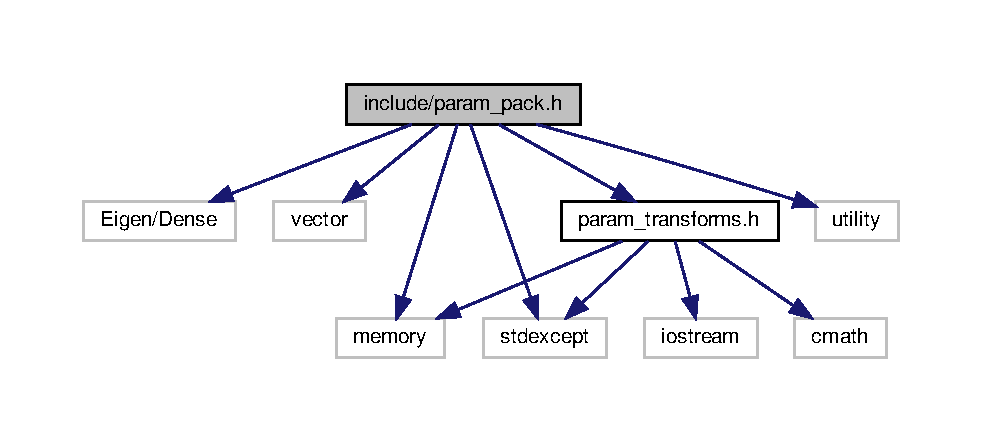
\includegraphics[width=350pt]{param__pack_8h__incl}
\end{center}
\end{figure}
This graph shows which files directly or indirectly include this file\+:\nopagebreak
\begin{figure}[H]
\begin{center}
\leavevmode
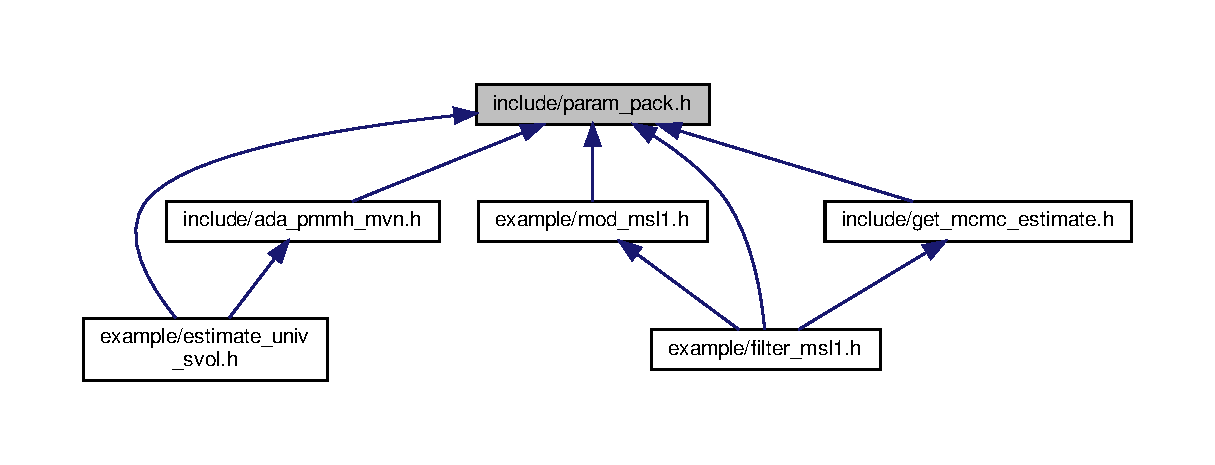
\includegraphics[width=350pt]{param__pack_8h__dep__incl}
\end{center}
\end{figure}
\subsection*{Classes}
\begin{DoxyCompactItemize}
\item 
class \hyperlink{classparamPack}{param\+Pack$<$ float\+\_\+t $>$}
\end{DoxyCompactItemize}


\subsection{Detailed Description}
Stores transformed parameters, as well as the functions that can change them to the untransformed parameters and back. 


\hypertarget{param__transforms_8h}{}\section{include/param\+\_\+transforms.h File Reference}
\label{param__transforms_8h}\index{include/param\+\_\+transforms.\+h@{include/param\+\_\+transforms.\+h}}


a pure virtual base class. cts params only.  


{\ttfamily \#include $<$memory$>$}\newline
{\ttfamily \#include $<$iostream$>$}\newline
{\ttfamily \#include $<$stdexcept$>$}\newline
{\ttfamily \#include $<$cmath$>$}\newline
Include dependency graph for param\+\_\+transforms.\+h\+:
\nopagebreak
\begin{figure}[H]
\begin{center}
\leavevmode
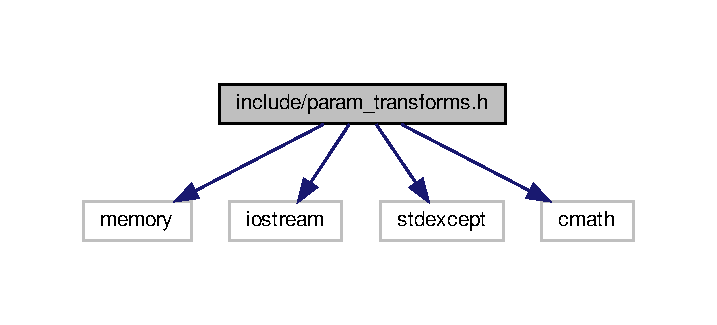
\includegraphics[width=344pt]{param__transforms_8h__incl}
\end{center}
\end{figure}
This graph shows which files directly or indirectly include this file\+:
\nopagebreak
\begin{figure}[H]
\begin{center}
\leavevmode
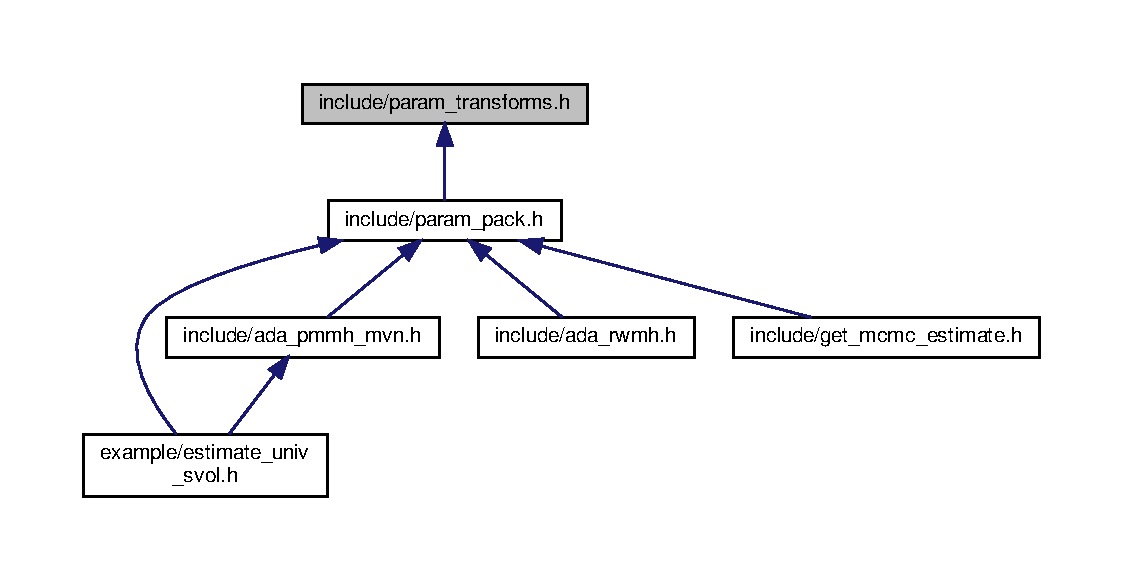
\includegraphics[width=350pt]{param__transforms_8h__dep__incl}
\end{center}
\end{figure}
\subsection*{Classes}
\begin{DoxyCompactItemize}
\item 
class \hyperlink{classparamTransform}{param\+Transform$<$ float\+\_\+t $>$}
\item 
class \hyperlink{classnullTrans}{null\+Trans$<$ float\+\_\+t $>$}
\item 
class \hyperlink{classtwiceFisherTrans}{twice\+Fisher\+Trans$<$ float\+\_\+t $>$}
\item 
class \hyperlink{classlogitTrans}{logit\+Trans$<$ float\+\_\+t $>$}
\item 
class \hyperlink{classlogTrans}{log\+Trans$<$ float\+\_\+t $>$}
\end{DoxyCompactItemize}
\subsection*{Enumerations}
\begin{DoxyCompactItemize}
\item 
enum \hyperlink{param__transforms_8h_acee593b112f4fc85f850631b9c6aaae9}{Trans\+Type} \{ {\bfseries T\+T\+\_\+null}, 
{\bfseries T\+T\+\_\+twice\+\_\+fisher}, 
{\bfseries T\+T\+\_\+logit}, 
{\bfseries T\+T\+\_\+log}
 \}
\end{DoxyCompactItemize}


\subsection{Detailed Description}
a pure virtual base class. cts params only. 

trans\+\_\+p = log(orig\+\_\+p).

trans\+\_\+p = logit(orig\+\_\+p).

trans\+\_\+p = log(1+orig\+\_\+p) -\/ log(1-\/orig\+\_\+p) = logit((orig\+\_\+p+1)/2).

trans\+\_\+p = orig\+\_\+p.

\subsection{Enumeration Type Documentation}
\mbox{\Hypertarget{param__transforms_8h_acee593b112f4fc85f850631b9c6aaae9}\label{param__transforms_8h_acee593b112f4fc85f850631b9c6aaae9}} 
\index{param\+\_\+transforms.\+h@{param\+\_\+transforms.\+h}!Trans\+Type@{Trans\+Type}}
\index{Trans\+Type@{Trans\+Type}!param\+\_\+transforms.\+h@{param\+\_\+transforms.\+h}}
\subsubsection{\texorpdfstring{Trans\+Type}{TransType}}
{\footnotesize\ttfamily enum \hyperlink{param__transforms_8h_acee593b112f4fc85f850631b9c6aaae9}{Trans\+Type}\hspace{0.3cm}{\ttfamily [strong]}}

enum class for different types of transformations 
%--- End generated contents ---

% Index
\backmatter
\newpage
\phantomsection
\clearemptydoublepage
\addcontentsline{toc}{chapter}{Index}
\printindex

\end{document}
